\chapter{How Do Home Computer Users Behave in Questionable Security Situations?}
\label{chap:ch3}
In this chapter, we present the findings from a human subject experiment that studied human behavior in practicing computer security.
In this study, we simulate cyber-security vulnerabilities that occur in a home computer environment when the human users perform routine tasks like checking email and using software applications. 
In our analysis, we find that the human users' intentions and post-hoc perceptions of computer security generally are not indicative of their actions; they were unaware when they had triggered security or privacy breaches.
The findings of this study motivated our work on plan intervention. 
In the next chapters we discuss three plan intervention models that can automatically detect an undesirable state developing and decide when to intervene.
Furthermore, our findings of this study support the claim that security solutions designed for end users to practice safe computing need to assess two information sources: 
\begin{itemize}
\item The human user's decision making context 
\item The factors that affect the user's decision making ability
\item Observational data like system logs and user action sequences
\end{itemize}

\section{Introduction}
The 2016 American Community Survey found that 89\% of all households had a computer, including smartphones, making it a common feature of everyday life \cite{ryan2016}. 
Also, 81\% had a broadband subscription. 
The Internet impacts many areas of the daily life; from performing routine tasks like shopping, banking and connecting with family and friends. 
The Internet has become an avenue for pursuing formal education (e.g., online degree programs) as well as informal learning (e.g., how-to videos on cooking, household repairs etc.) and allows us to collaborate across many physical barriers. 
Whether we realize it or not, we are routinely  deciding whether or not to take risks in security and privacy when we interact with computer systems online.

Home computer use, as distinguished from work related or organizationally based computer
use, is dominated by personal activities (mostly recreational, but some financial and health related) and is not governed by security policies determined by experts. 
Most security approaches for home users encourage them to take preventative or precautionary actions, such as installing anti-virus/malware software, hardening passwords \cite{chiasson2008}, backing up information \cite{dupuis2012}. 
In this study, our objective is to understand how home computer users
make more \textit{immediate} security and privacy decisions, such as whether to click on links in email messages, to install software or visit suspect websites. 

We distinguish two decision making contexts for home computer users: unwittingly taking action that may lead to undesirable consequences (e.g., clicking on links in phishing emails) and deciding to accept the possibility of undesirable consequences (e.g., financial transactions on trusted sites or P2P software installations). 
In the first case, the user does not recognize that the situation may have undesirable
consequences. 
Thus, our research in the ``\textbf{unwitting context}'' will be to initially assist the user in better identifying possible undesirable consequences of action. 
We will do this by designing methods for automatically recognizing security/privacy risks. 
We discuss intervention solutions that address this requirement in Chapters 4 and 5.
In contexts where the user recognizes the consequence, the research will address how to help users frame their decisions: determining what alternatives are available for the user to take as next steps.
We discuss an intervention solution that address this requirement in Chapter 6 of this dissertation.


While computer security and privacy decision making share characteristics of other decision making models about possibility of undesirable consequences, the combination of decision making models within the context of practicing cyber-security is unique. 
Thus, theoretical models (e.g., Protection Motivation Theory \cite{rogers1997} and Theory of Planned Behavior \cite{ajzen1991}) applied in other decision-making contexts (e.g., health) fall short in their applicability because they use different models of risk management. 
Because of the diversity of the population and decision contexts, we favor a personalizable approach in which computer assistance can be tailored to the individual user and the decision making context.


The study discussed in this chapter makes several contributions:
\begin{itemize}
\item Analyses and human subject studies relating what human users think is happening to what they actually do. This is critical to understanding how much information about user's decision making context can be inferred from surveys.
\item Studies and analyses relating perceptions, actions and some user characteristics to possible interventions.
\item Software framework to support home computer user security/privacy studies. We create a lightweight, sandbox software system, which simulates the Microsoft Windows environment on desktops and laptops. The simulator supports a small set of vulnerabilities and the scenarios that could possibly trigger them.
\end{itemize}

The decision of when to flag a problem for intervention also relies on the knowledge about the user. 
We refer to this as the \textbf{\textit{user's decision making context}}. 
Success of the intervention model will depend on not bothering the user unnecessarily. 

For example, consider cyber-security threats like phishing attacks and spoofing attacks.
If users have the skill for recognizing these cyber-security threats and understand the consequences, then they need less monitoring.
In contrast, users who are less aware of the computer security threats require more help. 
So, the question we need to address is \textit{what type of users make particular computer security decisions}. 
We answer this question by drawing from health related behavioral models to explain security behavior. 
Health behavior is a natural analogy to how human users respond to cyber-security threats. 
Human users frame many related issues in cyber-security using health related metaphors. 
For example, we refer to viruses and infections when talking about cyber attacks, we discuss system hardening after an attack takes place. 

The Health Belief Model (HBM) is focused on user's attitudes and beliefs. 
The user's beliefs are described based on their perceptions of six factors, susceptibility, severity, benefits, barriers, cues-to-action, and self-efficacy of performing a given health behavior \cite{rosenstock88}. 
In this work, we study the influence of two user characteristics when making security decisions from the HBM: \textit{self-efficacy}, that is an individuals confidence in her/his ability to perform a security enabling task on the computer, and \textit{cues-to-action}, that is an individual's response to external triggers for how they would affect users practicing computer security. 
We are adopting the HBM for studying user characteristics that affect computer security decision making because the HBM (specifically self-efficacy and cues-to-action) has been studied in prior work, which looked into computer security practices of the home user. 
Studies on self efficacy found that \cite{urbanska2013,aytes2004,milne2009} knowledge about how to practice safe computing increases the rate of safe behavior. 
However, having knowledge alone does not guarantee practice of computer security. 
For example, rapid advances in new security technologies make it harder for a user to keep up with the latest updates that must be made to ensure safety of his computer. 
Cues-to-action triggers are advice received from external entities like friends, co-workers, media reports, laws and regulations etc. 
Studies on cues-to-action \cite{claar2010,ng2007} find that these types of cues do not have a significant effect on human users practicing computer security.  
However, these studies mainly use self-reports to evaluate the effects of self-efficacy and cues-to-action on users' decision making. 
In this work, our objective is to find out whether the same effects can be observed from human users practicing computer security in a simulated home computer environment. Furthermore, the simulated environment allows us to present cues to users that can be monitored easily such as HTTPS/HTTP web sites and safe/unsafe hyperlinks. 
This enables us to measure user responses to measurable cues as opposed to cues obtained from external sources, which are often hard to monitor and control.

Considerable research has addressed human decision making about risk. 
An individual’s risk tolerance and perception is likely to be context specific; Weber et al. \citeyear{weber2002} divided contexts into: ethical, financial, health/safety, recreational and social. 
Computer security and privacy decisions share features of several of these. 
Like some health/safety decisions, the consequences may be delayed (e.g., information theft) or unnoticed (e.g., malware), the probability of risk may be perceived as low, the actions may be routine (e.g., reading email), and the immediate primary effects (e.g., playing a new game or looking at a photo of a relative) may be recreational. 
Unlike health/safety decisions, the cost of the threat is not as high (e.g., slow down of machine) or not as imminent (e.g., bot installed on machine). 
From the social context, the user may experience peer pressure to take some action and be unwilling to admit when something goes wrong. 
Like ethical decisions, risky actions may be violating laws (e.g., copyright in peer to peer file sharing) or putting others at risk (e.g., bots).
Additionally, the perception of cost for avoiding risk may be high (e.g., time spent learning about security), and the right actions may not be obvious (e.g., which security software to install or how best to make settings in browser). 
Moreover, given the disclosure of industry and government breaches, users may simply feel helpless.

In addition, the work by Davison and Sillence \citeyear{davinson2010} shows that human users' security related behavior often does not match their stated intentions. 
Human users often state the intention of being secure online but then perform actions that put their system at risk. 
Two studies \cite{govani2005, national2010} have been able to verify that the self reported values for some human user computer behaviors are in fact higher than the actual values.
This finding confirms that human users are unable to recognize  on their own that they need help while using computers, and would benefit from automated solutions that can help them during the decision making.
To this end, developing user-friendly security solutions requires observing users performing actions rather than relying on self reporting, which acts as a proxy for actual behavior. Ideally, the home computer user should be studied at home for an extended period of time to be able to accurately gauge the computer security related behavior patterns. 
However, these requirements pose many logistical and practical problems. 
For example, the software system used in such studies should be a background process with minimal intrusion to the user's normal computing activities while collecting the necessary system/behavior information at different levels of granularity (e.g., system calls, process information, user action sequences). 
Knowledge of having these computer security monitoring software installed in their personal computers may force users to practice computer security more thoroughly than they would normally, which will lead to artificial behavior data.  
Therefore, we need to balance collecting high quality information against privacy and practicality of studies. 
The sandbox environment  we present in this chapter is designed to address the problem of collecting reliable data from human users when practicing computer security. 
Using the sandbox environment the subject is asked to walk through a protocol (task list) in a controlled environment, in which they are presented with different decisions to be made and actions taken. 
The scenarios can be designed to test the effect of cues and responses of users, thus allowing us to study computer security practices without having to only rely on self reports. 



\section{Related Work}
Before effective interventions can be developed, we must understand what types of users make particular decisions, and how they prefer to make decisions. 
What are the factors that influence user's decision making? 
Studies that have tried to answer this question have used behavioral models as a guide. Like HBM, there are many other behavioral models that have been adopted to study human user behavior such as Theory of Planned Behavior \cite{ajzen1991}, Extended Parallel Process Model \cite{witte1992} and Precaution-Adoption Process  Model \cite{weinstein2002}. 
These models define constructs that collectively represent a person's actual control over the behavior. 
Studies that apply these models to explain user behavior in computer security have looked at computer security practices such as password management, email usage, backing up data, antivirus software and firewall usage in both home and organizational environments. Typically, the studies evaluate the effects of the model's constructs on practicing security using self reported surveys from human subjects. 
We now discuss human behavior models that are commonly adopted in studies about the home computer user's security behavior.


\subsection{Modeling User Behavior for Computer Security}
Users adopting computer security concepts share many similarities with how they respond in a health related scenario. 
For example, consider a user installing an antivirus software to protect his computer against malicious. 
This is very similar to someone adopting a healthy diet to avoid diseases. HBM was developed in the 1950s after the failure of a tuberculosis screening program attempted to explain and predict health behaviors. HBM consists of six core constructs that affect an individual's core beliefs on some health related concept. These constructs are: susceptibility, severity, benefits, barriers, cues-to-action, and self-efficacy of performing a given health behavior. Let us translate the HBM for a scenario where the user is trying to protect his computer against a virus attack using antivirus software. HBM states that the user's behavior will depend on the user believing that there is a high probability that his computer will be affected by a virus (susceptibility), the user believes that the negative effect of the virus attack is a serious problem for him (severity), the user believes that having an antivirus software is helpful in preventing virus attacks (benefits), the user believes that there is little difficulty in getting a good antivirus software and using it (barriers) ,the user believes that he can recognize external trigger events indicating the computer may be at risk (cues-to-action), the user believes that he is confident in his ability to install and use an antivirus software to protect his computer (self-efficacy).

HBM has been adopted in several studies about computer security practices of human users. Ng et al. \citeyear{ng2007} study the effects of HBM constructs operationalized to the security practice of exercising care when reading emails with attachments. They evaluate the effects of HBM constructs using self-reported behavior of users. Unlike our study, which focus on home computer users, this study is conducted in the organizational context. The study finds that when exercising care while opening email attachments, self efficacy, susceptibility and benefits are determinants of user behavior. They further find that barriers, cues-to-action and perceived severity are not significant determinants of security behavior. However, they note that although the cues they have evaluated (e.g., organizational awareness programs) are not effective in prompting secure behavior in users, other types of cues could prove to be effective. In our study, we intend to address this by evaluating cues that can be presented from within the computing environment (e.g., browser notifications, secure URLs) to promote secure behavior in users.

Claar et al. \citeyear{claar2010} studies the effects of HBM constructs in the context of using computer security software anti-virus, firewall, and  anti-spyware. Like our study, this study also focus on computer security behavior of the home computer user. Claar also extended the HBM by adding moderating variables gender, age, education, prior experience on the effect of computer software usage. Participants were recruited from university students and Internet groups and were administered a survey. The results show that self-efficacy, barriers, susceptibility influence computer security usage. This study also found that cues-to-action did not support how human users practice computer security.

Attack graphs \cite{ammann2002} have been proposed as a methodology of modeling how a security vulnerability (goal state) can be reached starting from an initial state through a set of state transitions. Urbanska et al. \citeyear{urbanska2013} propose an extension of the attack graphs that factors in the user's interactions  with the system (in addition to the attacker) that leads to the manifestation of vulnerabilities. This state/action model is referred to as a Personalized Attack Graph (PAG). The PAG provides a basis for answering two questions related to trigger identification: (a) Which are the ``appropriate'' system states that must be monitored? and, (b) Which user actions are predicted to possibly lead to a vulnerability? A PAG explicitly ties the dependencies between known vulnerabilities existing in a standalone system and the system configuration (including characteristics of the user), to the user activities, system actions and attacker actions that can lead to an exploit of a vulnerability. The personalized aspect of the PAG comes from incorporating information about the user as \textit{user attributes}. These attributes include, user actions, preferences and assets. The authors use a Bayesian network model influenced by HBM to assign probabilities to the user attributes. User attribute probabilities for a specific user is calculated from values assigned to the six primary factors in the HBM and six additional factors (prior knowledge, experience, gender, age, socio-economic and education). However, the PAG model is evaluated using synthetic data and expert opinion. In this work, we produce actual human subject data that can be used to accurately estimate these probability values for two of the HBM constructs: self-efficacy and cues-to-action.


\subsection{Challenges in Security User Studies}
Many studies on assessing human decision making in practicing computer security (including the studies cited in the previous section), report that one major challenge in conducting security user studies is the disparities between self-reported and actual observations. Howe et al. \citeyear{howe2012psychology} observed that most studies that look into computer security practices of users relying on self reported surveys suffered from issues such as respondent bias, socially desirable responding and peer perception. The authors posited that experiments based on simulation, which place the participant in the actual situation that is monitored can help reduce such issues and also be leveraged to assess the emotional reactions of users to interventions and warnings. 

Questions asked in self-reporting surveys induces respondent bias. For example in Ng et al.  \citeyear{ng2007}, the user is asked the question ``\textit{I am confident of recognizing suspicious email headers. (agree/disagree)}'' to measure self-efficacy. 
Users may find it difficult to estimate there skill level for some task and often overestimate their abilities. 
Furthermore, asking about computer security practices primes the user for security, which may be difficult for researchers to control. A human subject study that looked into effectiveness of SSL warnings that appear during Web browsing tasks \cite{sotirakopoulos2011} attempts to minimize the priming effect by designing tasks for the Web browsers the participants normally used and simulating the same look and feel of the native Web browsers. This study also used deception. The researchers did not reveal the true purpose of the study until the tasks were completed. The results of this study also confirms that there is a disparity between self-reported  and observed actions in computer security studies. We follow the same principles in our sandbox environment design and the administering the experiment. 

The sandbox environment has the same look and feel as the typical Microsoft Windows Desktop. We adopted deception by presenting the participants with a cover story, which stated that we were evaluating the participants on their ability to perform day-to-day computing tasks like checking email and web browsing. We also use a combination of surveys and observational data to identify predictors of user actions. Surveys are issued to participants at the beginning and at the end of the study to more accurately gauge what the users report and what they had actually done.

While the sandbox offers a controlled environment, it also affords realism and the ability to conduct longitudinal studies. 
This is particularly important in practicing computer security, which must continue beyond the initial adoption. 
Our sandbox study only looks into computer security practices in laboratory conditions and the study is administered only once. 
Accessing a user's computer in an unobtrusive way for a long period of time presents considerable challenges. Warkentin et al. \citeyear{warkentin2016} attempt to address this issue and presents a model that explains continuous intention to practice computer security. The researchers, measured the usage of an anti-malware software over nine weeks. The software was installed in the subjects' computers and usage data was sent to a web based server periodically. The study finds that in order to form an intention to continue the use of security software the effects of threat severity, susceptibility and self-efficacy are significant contributing factors.

Another challenge in human subject studies in computer security practices is the sample bias. Characteristics of the study participants vary from the general population of computer users.  Many studies use university students as the subject pool \cite{sotirakopoulos2011, warkentin2016} in order to draw a representative sample to the best of their ability. However, typical computer users are young, old, tech-savvy, non-tech-savvy, educated, uneducated, male, female and so on. The diversity of the sample should lead to more generalizable data. In our study, we also use the university students as a sample mainly because it is a sample of convenience. We however restricted the student sample to consist of non computer science majors so that we can better approximate an average home computer user.



\section{PsychoRithm: A Sandbox for Conducting Security Studies of Users}
We now present PsychoRithm, the sandbox environment we designed and implemented to study how the self-efficacy and cues-to-action impact security decision making of home computer users.
When running an experiment using PsychoRithm, the subject is presented with a desktop, which includes common applications such as emailing, Web browsing and file browsing. As the subject performs these activities, different events happen that can trigger threats and vulnerabilities of interest to the researcher. These events may include asking the user to register with a login name and a password, to provide sensitive information to gain access to a site, to respond to pop-ups asking the user to download a software. PsychoRithm records the user responses to these actions, including user clicks and time taken for response.

We had several design objectives. First, the environment needs to be as realistic as possible to encourage subjects to behave as they would on their home computers. When people are accustomed to using particular software, they have expectations about how to use it and what it will do. These expectations direct how they interact. Second, the software must be portable to different settings while also protecting the computational platform, allowing for simulation of security vulnerabilities without actually causing damage. We wanted a system that could be easily moved to a user location to run experiments. For example, if we wanted to study mature adults, we could take the setup to a senior center and conduct the experiments from there by installing the software on available platforms. Whether we run the study on someone's computer or our own, we need to retain control of the effects of the subject's actions. Yet, the possibility of infecting study machines with security experiments gone awry is very real. Given such constraints, we decided to create a fully simulated environment that would mimic the behavior of real world interaction without making any changes to the underlying operating system and minimizing changes to the file system. For example, if a pop-up asked the user to click on a button to download a software, the user would be able to click on the button, a download progress bar would show the changes, and finally a file icon would be placed in a mocked up file system browser to give the appearance that an actual file has been downloaded. Third, data collection needs to be computationally lightweight and privacy protecting. We considered a variety of methods for monitoring user interaction and found, unsurprisingly, that the most comprehensive are also the most computation intensive and potentially privacy invasive. We needed to strike a balance between carefully collecting/storing valuable data and damaging the privacy or the subject experience (e.g., not slowing down the computer so much that the subject notices). We now describe the tool we developed to support our controlled user study by first describing the user view and then the system view.

\subsection{Simulating Common Computing Activities in a Familiar Context}
Microsoft Windows is one of the most widely used desktop computing platforms accounting for 88\% of the market \cite{zdnet2020}. Thus, the look-and-feel of the Windows desktop and common applications is important to instilling familiarity for subjects. When a subject starts, he/she sees a Desktop as shown in Figure \ref{fig:desktop}. The Desktop provides application icons, e.g., a web-browser and a file-browser. Subjects can click these icons to launch the corresponding applications.

\begin{figure}[tpb]
  \centering
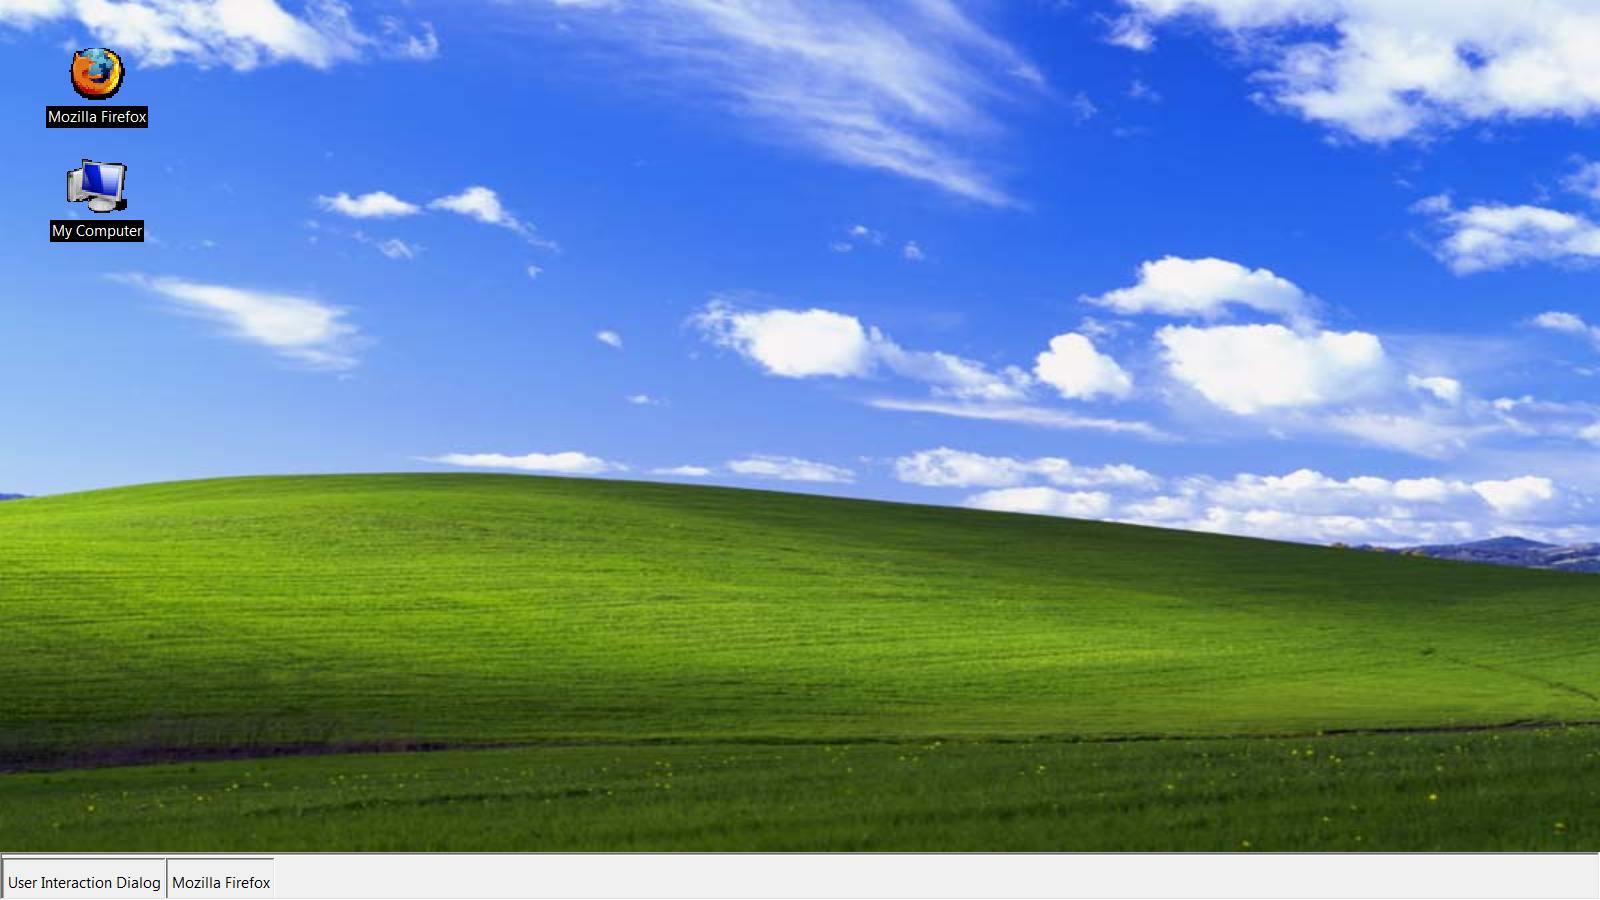
\includegraphics[width=\columnwidth]{img/desktop.png}
  \caption{Simulated Microsoft Windows desktop environment}
  \label{fig:desktop}
\end{figure}

In our study, the browser is the nexus; most of the interaction transpires through the browser. Subjects were instructed to open the browser which showed the starting page for the study (see
Figure \ref{fig:browser}). The browser not only guided the subjects through the tasks of the study, but also ensured that the subjects followed the required sequences. Subjects were allowed to perform a task only when the previous task was complete. For example, installing an application could not be skipped as subjects were required to post a verification code, which they obtained after running the application.

For the browser, we used FireFox (version 34.0.5) because it is open source, which allows us to customize the software to enable only the features we need for the simulated environment (forward/backward page navigation buttons, download button, address bar). To maintain the experience as being focused on computer interaction, web pages were used to collect pre and post interaction survey data. For our study, the data included demographic information as well as reports that could be compared against behavior as the subjects executed their tasks. To make the pages realistic, the URL bar in the PHP stub displayed the expected URLs (e.g., https://twitter.com) with an associated padlock to indicate that the HTTP connection was secure, when appropriate. The URL bar could be changed to test subject sensitivity to cues such as these. The browser also allowed for multiple tabs to be open for the experiment landing page and the various applications that are run within the browser.

Studies on global Internet users show that checking email, sending/receiving direct messages (chat), browsing for information/research and social media activities account for the bulk of the online activities \cite{furnell2007, worldinternet2018}. Thus, simulating these activities was a priority for our tool; the current version includes simulated applications of email and Twitter. Because ``google and click'' is so open ended, we did not include it in the current version of the tool.

\begin{figure}[tpb]
  \centering
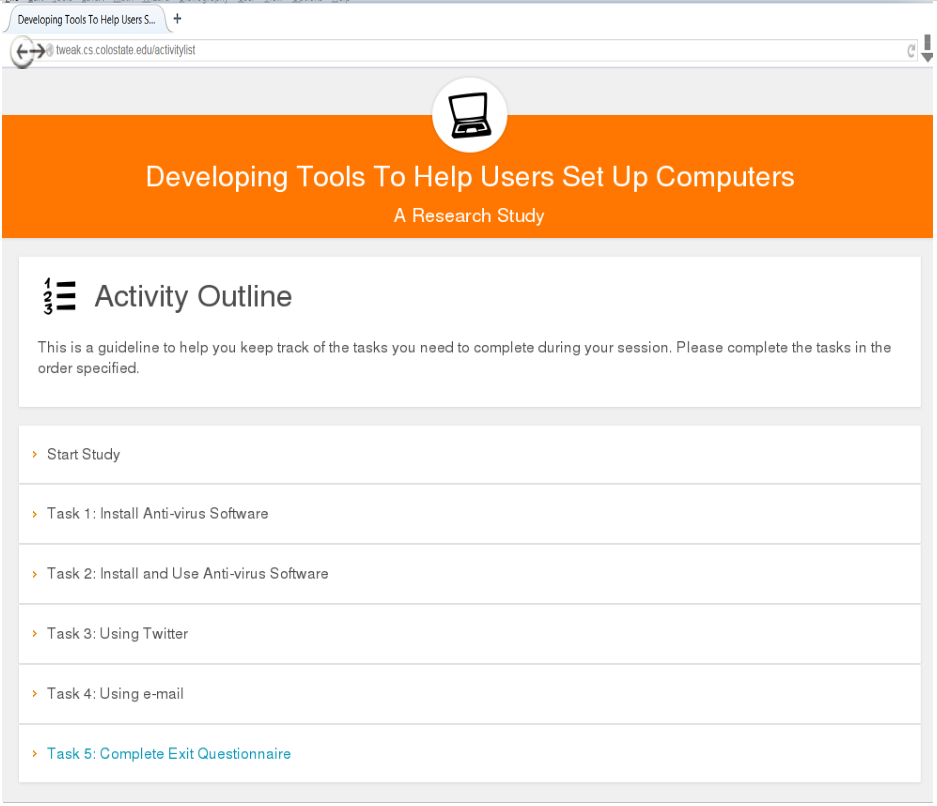
\includegraphics[width=\columnwidth, keepaspectratio=true]{img/browser.png}
  \caption{Simulated Mozilla Firefox Web browser}
  \label{fig:browser}
\end{figure}

Our email application was based off of SquirrellMail (version 1.4.22). SquirrelMail includes built-in PHP support for the IMAP and SMTP protocols and all pages render in pure HTML. These configurations fit perfectly to the technologies behind our simulated environment and therefore we could easily integrate it as an add-on service to the desktop environment. Our version of mail supports login and message functions. Subjects login using provided usernames and passwords and then can change their password. They can look at a list of messages, read and answer them. For purposes of this study, the email accounts can be populated with a set of email messages. Figure \ref{fig:mail} shows three emails that were used in our study and that were related to the other applications in the experiment protocol.
\begin{figure}[tpb]
  \centering
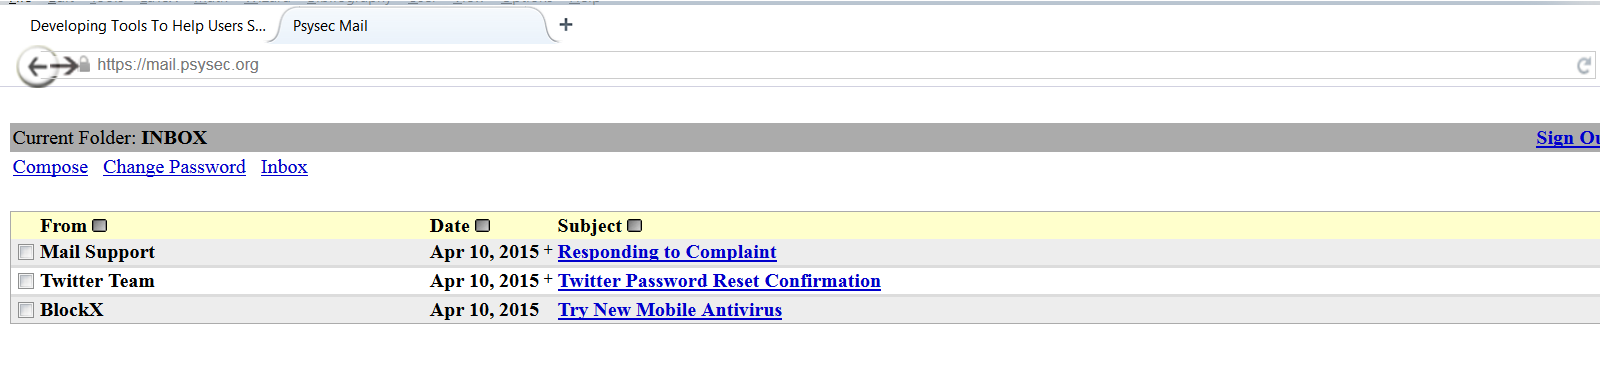
\includegraphics[width=\columnwidth, keepaspectratio=true]{img/mail.png}
  \caption{Simulated SquirrelMail email client}
  \label{fig:mail}
\end{figure}

As with email, our Twitter application supports login and message functions. Each participating user was provided with a twitter handle and a password. Three messages were posted in their respective Twitter inboxes (see Figure \ref{fig:twithome}). One of the three messages as shown in Figure \ref{fig:twitmsg}, which appears to link to a phishing website; if they click on the link, they are taken to a site which requested subjects to provide their Twitter username and password. 
\begin{figure}[tpb]
  \centering
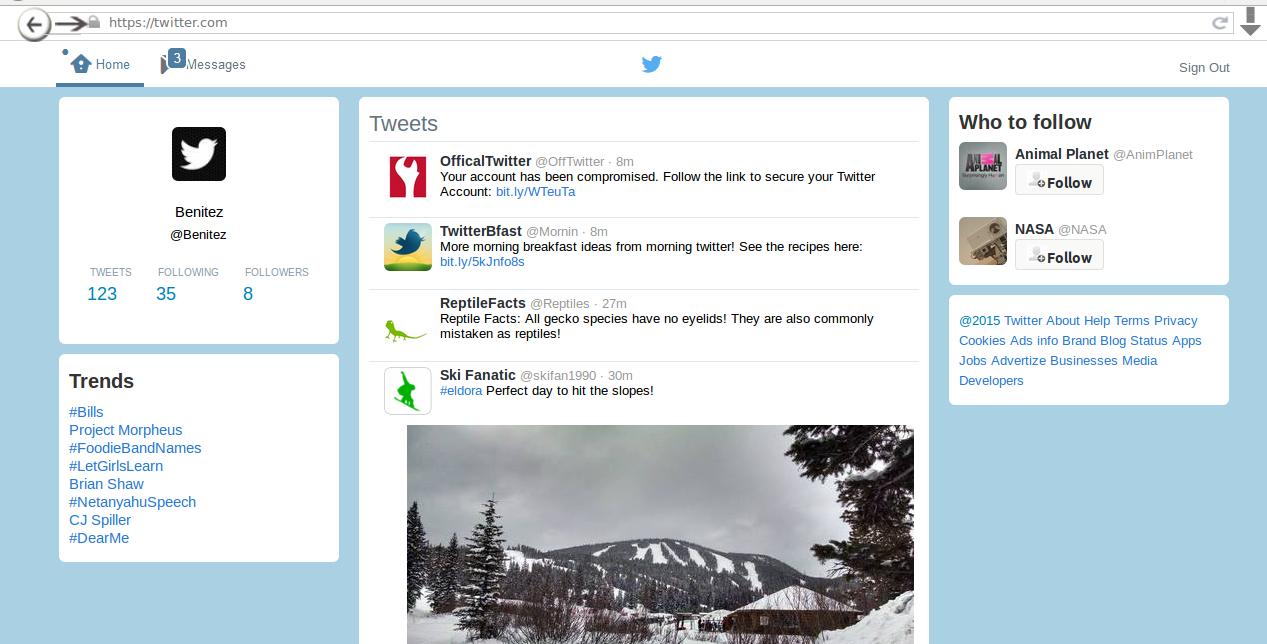
\includegraphics[width=\columnwidth, keepaspectratio=true]{img/twitterhome.png}
  \caption{Simulated Twitter home page with three direct messages in the inbox}
  \label{fig:twithome}
\end{figure}

\begin{figure}[tpb]
  \centering
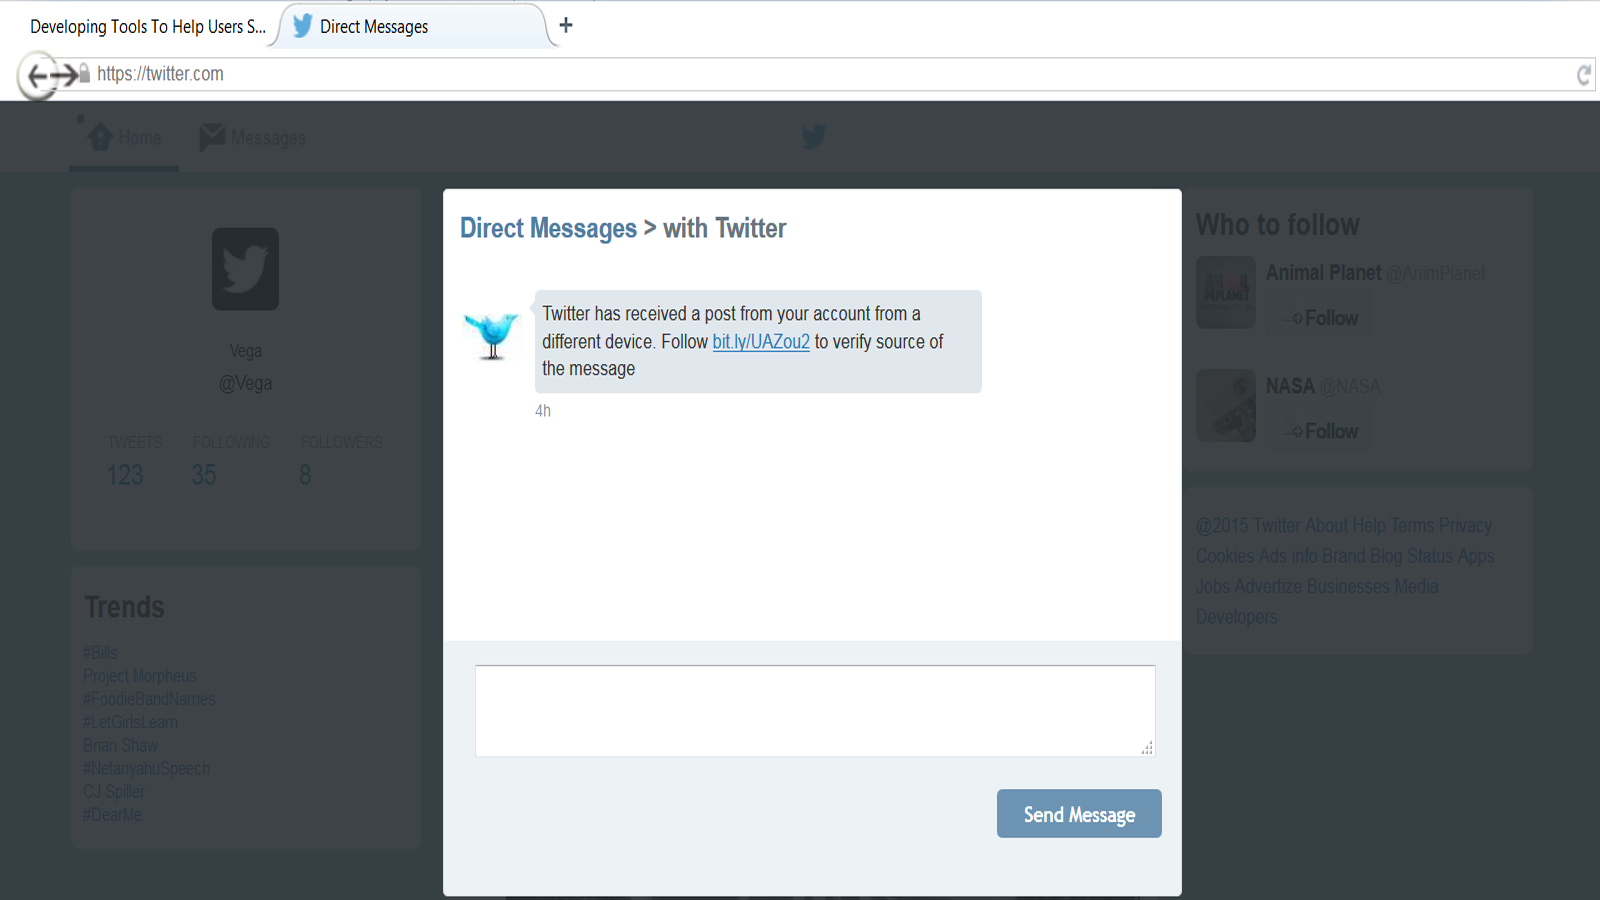
\includegraphics[width=\columnwidth, keepaspectratio=true]{img/twitter.png}
  \caption{Simulated Twitter direct message}
  \label{fig:twitmsg}
\end{figure}

To monitor the user's aptitude to use a common software application, we included an anti-virus software selection and installation activity. The subjects accessed an anti-virus download portal which leads to two separate websites as shown in Figure \ref{fig:virus}. One of the web-sites was purposefully made secure (HTTPS) while the other was made to look like a typical phishing site with flash images and dramatic warnings. Once the applications were downloaded, the subject was notified of the completed download. The subjects were then required to install and/or run the applications. To make sure the subjects installed and ran the downloaded application, the portal requested a verification code which was obtained by running the downloaded applications. Both anti-virus `downloads' were equipped with simulated system scanning capabilities (e.g., a progress bar appearing after the system scan is started).
\begin{figure}[pbt]
  \centering
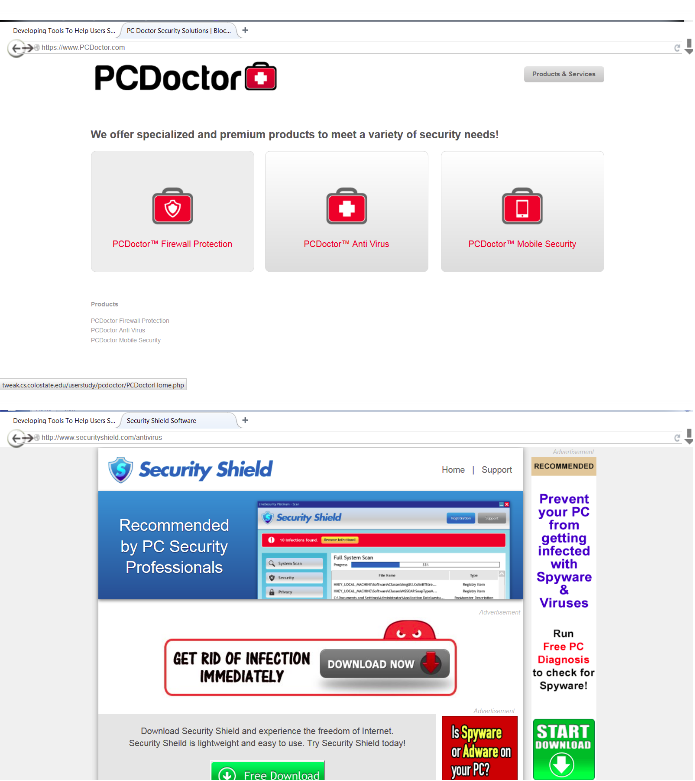
\includegraphics[width=\columnwidth, keepaspectratio=true]{img/virus.png}
  \caption{Simulated Anti-virus download pages: secure anti-virus software (top) and unsafe anti-virus software (bottom)}
  \label{fig:virus}
\end{figure}



\subsection{System Architecture}
The PsychoRithm software was designed to operate as a kiosk. The software creates a Simulated Local Environment on the subject's machine. The required applications such as the email program, the Twitter site, anti-virus software web pages, phishing web pages, and the survey questionnaires reside on the server. Software architecture diagram for PsychoRithm is shown in Figure \ref{fig:psyarch}
\begin{figure}[pbt]
  \centering
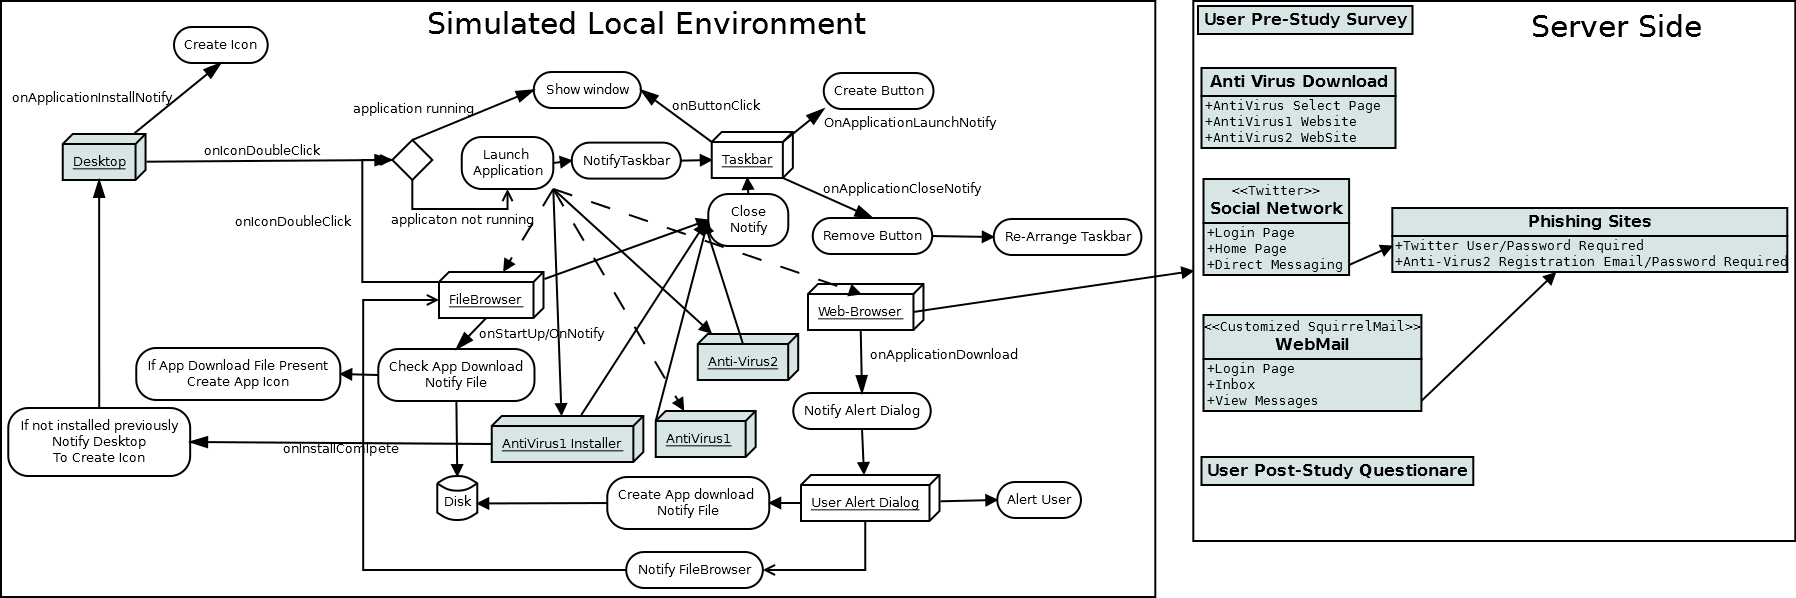
\includegraphics[width=\columnwidth, keepaspectratio=true]{img/fulluml.png}
  \caption{PsychoRithm software architecture diagram}
  \label{fig:psyarch}
\end{figure}


\subsubsection{Desktop and File System}
The user interacts with the desktop and the file system to download, install and run applications.
At the start of the experiment, the user validates his experiment username with the desktop,
and the desktop creates a folder specifically for that user. The simulated desktop provides application icons: Mozilla FireFox Web browser and the My Computer file browser (Figure \ref{fig:desktop}). The user can click these icons to run the corresponding application. When new applications are installed, such as the anti-virus software, new icons are added to the desktop. The desktop and all applications are supported by a taskbar, which provides easy access to all opened applications.

To make the simulated desktop resemble a real desktop, we implemented it as the topmost Win32 Tool Window spanning the working area of the actual desktop. Underneath the simulated desktop is an invisible list-view window, which hosts the application icons. Inter-process communication was performed using custom defined messages with application specific WPARAM values. We implemented our own opaque taskbar as a Win32 Toolbar that maps a zero-based incremental index to the launched applications. This index was used to track buttons/window-handles and close/rearrange them when applications were closed.

PsychoRithm was built as a package that contained empty folders like the \textit{Downloads} and \textit{LoginData}. It was placed under the \verb|C:\Users\<login_name>\Documents}| directory (to avoid conflict with system directories) and identified with \verb|login_name| on the fly to create the absolute path to the package. However, since the path was created dynamically, we could not configure the exact location of the \textit{Downloads} folder into Firefox and hence used the \textit{User Alert Dialog}. A Win32 window with an underlying list-view was used as the file browser for the \textit{Downloads} folder.


\subsubsection{Web Browser}
The Web browser component allows the user to browse the content fetched from the server. To create the illusion that applications were downloaded from a specific URL, we disabled the Firefox warning dialog by editing the mimeTypes.rdf which led to Firefox calling the User Alert Dialog. Similarly, to make websites like Twitter appear to be served from twitter.com, we removed the URL bars from the existing Firefox application and introduce a custom PHP stub (enabled with Javascript navigation functions) which emulated a URL bar and allowed subjects to navigate/reload pages in same browser session. This required mocking up images that made the interface appear as expected and means that any visited URL must have a corresponding image to be loaded. Action login was facilitated by PHP session variables and AJAX event handlers.

All widgets were disabled using a FireFox extension. When subjects double-clicked on the Firefox icon, the Firefox window was brought above the simulated desktop window giving the illusion that a new application has been launched. A custom designed Firefox extension allowed subjects to minimize this window, but not quit it.

\subsubsection{Email}
The SquirrellMail portal ran on top of a DoveCot IMAP/POP3 server.

\subsubsection{Anti-virus Applications}
Two anti-virus applications were created using Java Swing Platform. One of the anti-virus applications requires installation. After installation, it notifies the Desktop, which then creates an icon
to launch the application. To make the download process realistic, the web browser makes a call
to the \textit{User Alert Dialog}, which then alerts the user, creates a 0 byte file in the Downloads folder
and notifies the file browser.

\subsubsection{Collecting Data}
The system is instrumented to collect subject actions, specifically the start and conclusion of the session, the activation of each activity, typing and mouse clicks in the applications (buttons, widgets, windows, etc.) The results of the pre and post surveys and subject preferences (e.g., software selections, password choices) were also logged using PHP session variables. All activity related data are captured with timestamps. Once the experiment is complete, the Desktop
process sends over all captured data to the server side using SFTP/SCP, cleans all of the local storage and kills any process that was initiated by the system.

As per the regulations of the Institutional Review Board (IRB) of the Colorado State University, the researchers are required to store subject data in a safe and secure manner. Moreover, to run enough subjects, we needed to allow multiple subjects to participate simultaneously. Consequently, a secure remote server also stored experiment data in a safe manner. To preserve anonymity, the data were associated with the IDs (login names), which were assigned randomly when subjects arrived for the study and were never associated with specific individuals.

\subsubsection{Configuration and Extensions for Other Studies}
\sloppy
Microsoft Windows and Visual Studio Framework are required to install and use PsychoRithm. 
The web applications (Twitter, Antivirus Software Download) pages are implemented using HTML/AJAX/JQuery. 
The Anti-virus mock-up software is implemented using Java. 
For this study, the simulator only supports Web browsing (restricted only to predefined URLS), file browsing (restricted only to personalized \textit{Downloads} directory) and email (restricted only to SquirrelMail webmail application) applications. Access to other Windows applications are restricted through the simulated desktop and the web application shown in Figure \ref{fig:browser}. 

Because Firefox is an existing application, it must be started at the beginning of an experiment session and cannot be stopped during the course of the experiment. 
As a result, the subjects were only allowed to minimize the application and restore it via the taskbar button. 
All menu operations, including right-click menu operations, were disabled. 
In this study, our main focus is on evaluating users' behavior with regard to self-efficacy and cues-to-action while performing common tasks on the computer. 
There are other behavior models describing many other factors that affect user's computer security behavior. 
When evaluating the factors beside the two we are testing in this study, in their real usage context, the simulator software may require extensions for additional, more complicated tasks. 
In this case, future add-on Windows applications can be developed using the aforementioned technologies and integrated as plug-ins.


\subsection{Studying Behavior In Situ}
The goals of this experiment are:
\begin{itemize}
 \item capturing actions taken by users when asked to perform tasks that provided ``opportunities'' to trigger security vulnerabilities
 \item characterizing their behaviors by their gender and prior experience
 \item assessing consistency in subjects answers
and actions.
 \end{itemize}
In this study our focus was on two factors common to several well-known models of user security behavior: self-efficacy and cues-to-action (e.g., Health Belief Model, Protection Motivation Theory). The core idea was to ask questions related to those two factors, then observe the user actions within scenarios designed to elicit potentially detrimental responses and then to ask questions about the tasks that they had undertaken. This protocol was designed to collect data on how the two factors manifest in the participant sample and to allow us to compare the self reports of against the observed actions. While we had no hypothesis about how the factors would appear, our hypothesis about the comparison of data collection methods is that self-reporting was likely to differ from observed actions. Thus, the study was designed with five parts: an introduction, a pre-study questionnaire, on-line completion of four tasks, a debriefing and a post-study questionnaire.

The sandbox software allowed us to analyze the actual behavior of human users when they are presented with scenarios that may lead to serious computer security exploits such as installing illegitimate software, responding to phishing email, not changing default passwords, potentially in contrast to what they report in a survey. If the participants were directly informed of the real purpose of the study (i.e., computer security practices), it is likely they would be extra cautious in completing the tasks. This self-consciousness could influence what they do in the experiment making it differ markedly from their actions outside the context of the research study (e.g., at home, workplace) and introduce an additional bias to measurements we collect. To this end, we introduced some deception into the study in three ways:
\begin{enumerate}
\item The description of the study used to attract participants indicated that the study was to evaluate their ability to complete common tasks on the computer so that the researchers can
use the findings to develop tools to help users set up their computers.
\item A task, which was unrelated to the focus of the study (i.e., compose and save email as draft)
was added to one of the other tasks to help mask the actual purpose of the study. This task
did not generate any useful data.
\item To induce a sense of buy in, the participants were presented with a cover story at the start of
the study. The cover story stated that the participant had purchased a second hand computer
with Microsoft Windows and one utility application (Mozilla Firefox) installed. Experiment tasks were to study the participants ability to set up this newly purchased computer to be used as an additional computer by multiple users at their home. The cover story was
communicated to participants during the introduction session.
\end{enumerate}
During the debriefing session, participants were informed of deception used in this study. The study was designed as a within-group experiment, where all participants were placed in identical threat scenario simulations. Written instructions were given to all participants to assist them in completing the required set of tasks. All data were collected through the PsychoRithm sandbox. Text computer logs recorded the tasks that were completed, timestamp at which a task was completed, the selections made when options were presented, external URLs visited by following links on web pages, and updates made to user visible settings. Video/audio recordings were not used. The study took approximately 45 minutes to complete.


\subsubsection*{Participants}
In Spring 2015, we collected data from 61 university undergraduates as participants. The students were enrolled in a psychology course during that semester. The course attracts a wide range of majors and gives research credit for participating in studies. All participants were given informed consent and participated voluntarily.

Although selected as a sample of convenience, the sample was representative of home computer users from a critical group: young adults with easy access to computers. Prior studies have shown that high school and college aged adults, age between 18 and 34 report the highest level of Internet usage \cite{census2012}. 56\% of participants in this study were female. 74\% were less than 20 years of age, 25\% were aged 20-25 years and the remaining participant was aged 26-30. 98\% were working toward a Bachelor's degree.

\subsubsection*{Surveys}
We presented two surveys. The pre-study survey shown in Appendix \ref{apx:cypre} asks three questions (questions 1 - 3) about demographics and 10 questions about computer experiences (questions 4 - 13). Although we would have liked to directly assessed self-efficacy, the standard questions, as pioneered by \cite{ng2007, claar2010}, asked about level of confidence when executing specific tasks in different contexts. We did not wish to prime the participants to be thinking about computer security during the on-line portion of the study. Instead, we followed the tone of Mannan and van Oorschot \citeyear{mannan2008}, which asked about their experience with computers (questions 4 - 8), what challenges they perceive (question 9), where they obtain help (questions 10 - 11) and what software they have installed (questions 12 - 13). These questions were selected to relate more clearly to the cover story.

For the post-study survey shown in Appendix \ref{apx:cypost}, we adopt the standard survey instruments, which evaluate self-efficacy for computer security practices from \cite{ng2007, compeau1995}. Instruments that measure cues-to-action are adopted from \cite{ng2007}. It must be noted that our idea of cues refer to security notifications available in the computing environment such as SSL lock icon in URLs, web site content/look and feel as opposed to external information sources like news, help-desks etc. in Ng et al.\citeyear{ng2007}. Questions 2 - 11 evaluate the self-efficacy of the anti-virus software usage. Questions 12 - 19 evaluate self-efficacy of safe communication over social media (Twitter). Questions 21 - 24 evaluate self-efficacy of using email and managing passwords. Questions 20, 25-29 are about awareness of secure and private information collection. Questions 30 - 35 evaluate cues-to-action on practicing computer security on the Internet. The first question asks for the pseudonym which allows us to connect the on-line portion's data with the post-survey data. The main purpose of these questions was to establish whether or not the actions in the online portion of the study corresponded to what they thought that they did.


\subsubsection*{Experiment Procedure}
When the participants arrived for the study, one person checked their name on an attendance list, and then another person had them pick a persona ID from folded slips of paper in a basket. The persona ID included a fictitious name, user ID and password to login to the simulated desktop. All data were collected using the persona ID, which was never connected back to the participant's actual name. They were then led to a computer and assisted in logging into the kiosk software.

The starting page provided the instructions to the participants. To avoid alerting them to security issues, we presented the cover story below for what they were being asked to do.

\begin{center}
\framebox{%
  \begin{minipage}{0.8\columnwidth}
    \setlength{\parindent}{25pt}
    You have just bought a second-hand desktop computer from Surplus Property, the recycle, reuse sales point of Colorado State University. This computer will be used as an additional computer at home. The computer already has Microsoft Windows operating system installed. Notepad, Windows Media Player and Mozilla Firefox web browser are installed as application software. Additionally, you also managed to get an Internet connection setup for the computer. This computer will be used by you and your family members for regular purposes such as checking email, browsing Internet, and also for entertainment activities like watching movies and videos.
    
  \setlength{\parindent}{25pt}
This study helps us understand your ability to perform common tasks on a computer, while it is being set up. To familiarize yourself with the new environment, you may browse the computer and check what applications are installed. Please note that, for the purpose of this study, a custom desktop environment was created and therefore it may not have all options available in a typical desktop computer.
\end{minipage}}
\end{center}

\vspace{1em}
The participants were presented with a screen that described and organized their on-line tasks. This page was generated as the participant finished one activity and moved on to the next. They were first directed to take the pre-study survey. Their last task was to complete the post study survey. The online portion presented three threat scenarios: (1) selecting, installing and using an antivirus software to ensure safety of the computer, (2) communicating on social media and (3) using email.

In the first scenario, participants were directed to install, configure and run anti-virus software as part of setting up their new machines. Below is the the instructions that were presented to the user as they started these tasks.
\begin{center}
\framebox{%
  \begin{minipage}{0.8\columnwidth}
  \textbf{ Task: Install Anti-virus Software}\\
  \setlength{\hangindent}{15pt}
	\textit{Please read the following description before you begin.}
	
	\textit{You may have noticed that the computer does not have any anti-virus software installed. You are concerned about this lack because the computer will be shared among your family members. Your  task is to install and configure an anti-virus software to be used in this computer. Names of software you will see during tasks are fictitious.}

	\begin{itemize}[topsep=8pt,itemsep=4pt, parsep=-4pt]
	    \item \textit{On ``Study Road Map'' web page click ``Install Anti-virus Software'' Link. You will be directed to a page with two anti-virus program options: \textbf{PCDoctor}, and \textbf{Security Shield}}
    \item \textit{Read the descriptions given for each software}
    \item \textit{Choose ONE anti-virus program. On clicking ``Visit web page to Download Now'', you will be directed to software provider's web page.}
    \item \textit{Find the correct download link on the provider's page. }
    \item \textit{Click on the correct download link to automatically download the software onto your computer.}
    \item \textit{Run installation wizard to install the software on your computer.}
	\end{itemize}

\end{minipage}}
\end{center}

Two antivirus software installations were offered via a web-based download portal implemented within PsychoRithm. One software was designed to be legitimate and safe; the other was intended as suspect and insecure. Neither were existing products or websites; in each case, we patterned our fictitious web pages after exemplars of each type of antivirus software website.  The legitimate software is ``PCDoctor'', and the suspect one is ``Security Shield''. The portal provided a brief description about each software program to assist users make a decision about which program to download. Once the software was downloaded, users were given written instructions to install the software, configure it to enable three additional security features (automatic live updates, removable media scan, and smart firewall) and finally perform a simple scanning task on the computer. Although neither program actually did anything, both were designed to give the users the interaction experience of an authentic antivirus program with appropriate timing pauses and messages (see Figure \ref{fig:rogueav}).  

\begin{figure}[!pbt]
  \centering
  \subfloat[System scanning]{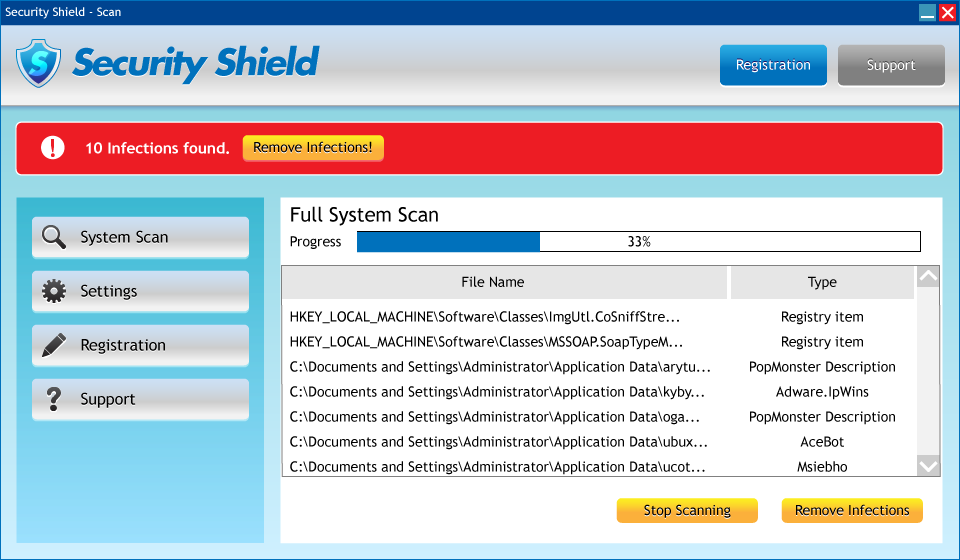
\includegraphics[width=0.5\columnwidth]{img/av1.png}\label{fig:scan}}
  \hfill
  \subfloat[Anti-virus protection settings]{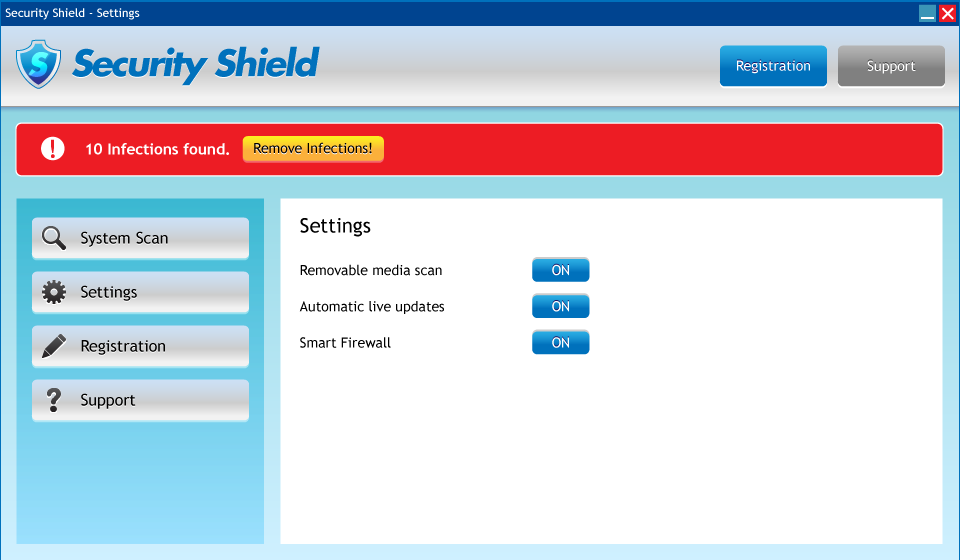
\includegraphics[width=0.5\columnwidth]{img/av2.png}\label{fig:settings}}
  \caption{Security Shield anti-virus mock-up software}
  \label{fig:rogueav}
\end{figure}

A mock-up version of a popular social media application (Twitter) was implemented for the purpose of studying users' communication habits. In this activity, users were instructed to use a private messaging feature of Twitter. In this case, we did create an version of the interface for the specific media site because it corresponded well with the cover story and we were interested in their behavior within this likely familiar context. Users were shown three private messages: two legitimate, safe messages sent from trustworthy sources (different offices within the university at which the study took place) and one phishing message. As shown in Figure \ref{fig:twitmsgall}, all messages contained URLs. The URL in the phishing message, directed users to a phishing website \texttt{bit.ly/UAZou2}. Once the users visited the phishing website, they were prompted to enter their username and password. In their instructions, they were told that this task would allow them to check that Twitter was working correctly on the computer; they were asked to login, read messages and ``take appropriate action''.

\begin{figure}[pbt]
  \centering
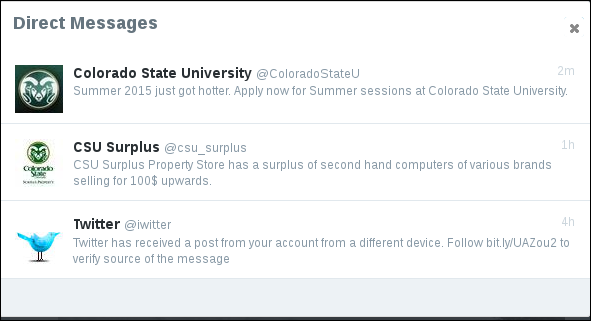
\includegraphics[width=0.7\columnwidth, keepaspectratio=true]{img/twittermsgs.png}
  \caption{A screenshot of the messages as they appeared to the participants}
  \label{fig:twitmsgall}
\end{figure}

A web based email client was used for the email scenario. Users were given personal email accounts and a common default password designated for the study. They were told ``The email account is unique to you. However, the default password is being shared by all users of the computer.'' The email task comprised two sub tasks. First, to study their ability to choose strong passwords, participants were instructed to change the default password of their email accounts to a new password of their choice. Second, users were instructed to compose a new email message, read email messages and respond to unread messages.

As shown in Figure \ref{fig:emails}, three new messages were placed in the inbox: one safe message and two unsafe messages. One of the two unsafe messages was a phishing message with a URL that would direct the user to a phishing website upon clicking. The phishing website was masked as the web-mail client itself. The other unsafe message contained an attachment: a harmful zip file. The message content was patterned after actual phishing email messages. The phishing websites and zip file attachments were mock-ups within the sandbox; thus, they did not pose an actual security threat to the computer or to the participant's personal data. 
\begin{figure}[tpb]
  \centering
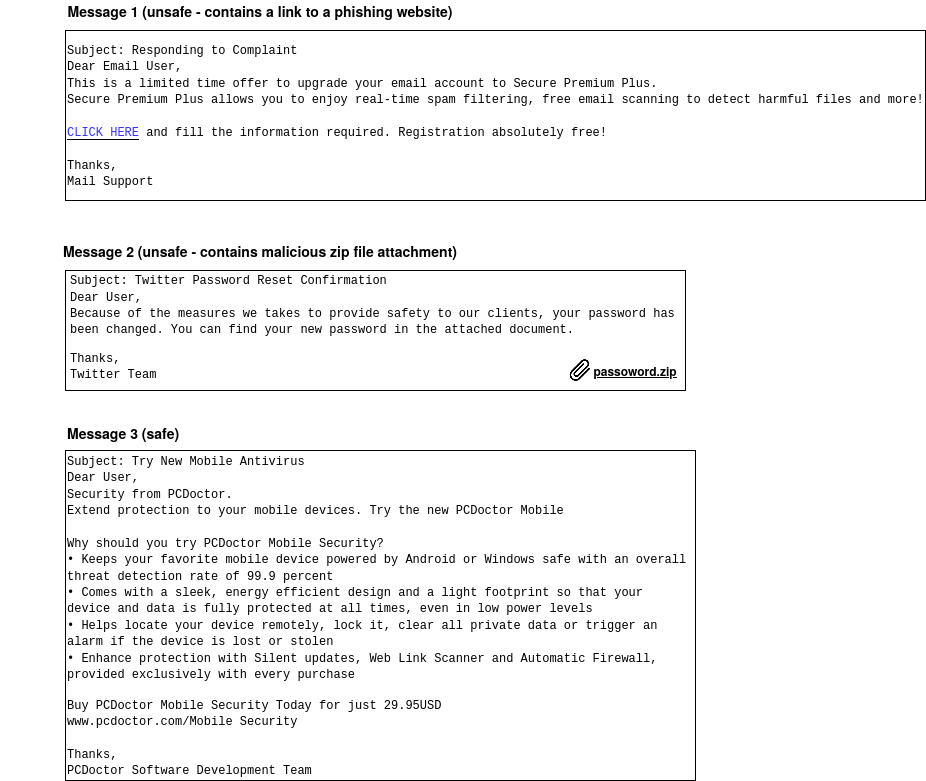
\includegraphics[width=\columnwidth, keepaspectratio=true]{img/emails.png}
  \caption{Email messages presented as part of the online portion of the study.}
  \label{fig:emails}
\end{figure}

We designed the phishing website to follow examples we had seen before and also placed several cues in line with commonly recognized properties of online phishing attacks \cite{ftc2019} for both the social media phishing attempt and email phishing attempt. First, in the case of Twitter, although the message sender's name was ``Twitter'', the Twitter handle (i.e., message sender's twitter account name) was not similar to the legitimate Twitter account's Twitter handle. The legitimate account's Twitter handle is \texttt{@Twitter}. The phishing message was sent from the Twitter handle \texttt{@iwitter} (i.e., Twitter misspelled). Second, the message said that some log-in attempts have been noticed. Third, the message content requested that the recipient confirm some personal information, specifically the user's Twitter account user name and password. If the user failed to recognize these cues and clicked on the link, the user is directed to a web page, which contains a log in page but looks different from the legitimate Twitter login page. Users had already seen the legitimate login page at the start of the Twitter task and ideally should be able to recognize that the current web page is different. We added several cues to this page as well. We changed the Twitter logo and the color scheme of the phishing web page. The URL did not contain the SSL lock icon and was \texttt{http://iwitter.com}, whereas the legitimate web site's URL was \texttt{https://twitter.com}. If the user did not recognize the phishing web site given all these cues and submitted the user name and the password, the user was directed to a landing page, which displayed a message that the user's personal information has now been compromised. Then the user was directed to the next task.

A similar approach was taken to handle security attacks that occur via email. The phishing message on email was masqueraded to appear as if it was being sent by the Anti-virus software vendor. Recall that, in the sequence of tasks, when the user reaches the email task, they would have already completed the anti-virus task and is familiar with the Anti-virus vendor's name. We embedded the same discrepancies between the legitimate vendor's information and the phishing website as the Twitter phishing scenario as cues for the email phishing use case. If the user clicked the phishing link, the same sequence of events took place as in the case of the Twitter phishing scenario. There were several cues to recognize the malware email such as the generic greeting from the sender (``Dear User''), an enticement to open an attachment (get the new password by opening the attachment), information review check (password change) and undisclosed recipient (``Mail Support''). If the user clicked the attachment, the user was directed to a web page, which displayed a message that the computer system's safety is now compromised.


Once the participant finished the tasks, he/she was directed to the post-study survey and a
debriefing explanation. We also offered them the opportunity to further discuss the debriefing with one of the staff conducting the study.


\section{Data Analysis and Results}
This study has two main components that evaluate users' computer security behavior: self-report surveys and the sandbox activities. Therefore, we divided the analysis as within component (only surveys and only sandbox) and across component (surveys and sandbox). We first present the analysis on single components.

\subsection{Pre-Survey Findings}
The survey can be found in the Appendix~\ref{apx:cypre}, page~\pageref{apx:cypre}.
Table \ref{tab:cypre} shows a summary of the pre-survey findings. 
Although the participants had a lot of prior experience with computers (66\% with more than 9 years), they had little formal training (59\% had none) and turned to the Internet for help as their primary source (92\%). 
Most (82\%) owned multiple devices. 
Nearly all (95\%) had installed multiple applications, i.e., Chrome, Office, Flash, Skype and Acrobat. 
Given the participant recruitment method, it was not surprising that nearly all had laptops and used their computers for educational activities. With respect to computer security, more than half (67\%) found it challenging to identify harmful actions and take steps to ensure safety. 
Yet most (77\%) had anti-virus software on their computers.

\begin{table}[tpb]
 \caption{Summary data from the pre-study survey questions. Each row is a question with its number and short description. Highest values in each row are in bold.}
\label{tab:cypre}
 \resizebox{\columnwidth}{!}{
\begin{tabular}{|ll|}
\hline
Years experience &
  4-6: 11\%, 7-9: 23\%, \textbf{\textgreater 9 : 66\% }\\ \hline
Usage hrs/day &
  \textless 3: 30\%,\textbf{3-6: 54\%}, 7-10: 11\%, \textgreater 10: 5\% \\ \hline
Devices &
  \begin{tabular}[c]{@{}l@{}}\textbf{laptops: 97\%}, smartphones 82\%, tablets: 33\%, desktop PCs: 21\%, \\ e-Readers: 7\%, Other: 3\%\end{tabular} \\ \hline
Applications &
  \begin{tabular}[c]{@{}l@{}}\textbf{web browser: 98\%}, Office: 82\%, Acrobat: 61\%, Media Player: 49\%, \\ Computer Games: 26\%, \\ Image Processing: 21\%, Software Development: 11\%, Other: 3\%\end{tabular} \\ \hline
Purposes &
  \begin{tabular}[c]{@{}l@{}}\textbf{Education: 93\%}, Documents: 84\%, Communication: 82\%, Entertainment:\\ 82\%, Information gathering: 74\%, Financial: 56\%, Work: 41\%, Games:\\ 26\%, Programming: 10\%\end{tabular} \\ \hline
Challenges &
  \begin{tabular}[c]{@{}l@{}}\textbf{Identifying actions that may harm the computer: 67\%}, Taking steps\\ to ensure the safety of the computer: 51\%, Installing, configuring and getting\\ a software application ready to be used: 43\%, Finding application software\\ that matches my requirements: 39\%, Finding and using help manuals: 25\%\end{tabular} \\ \hline
Training & 
\begin{tabular}[c]{@{}l@{}}\textbf{None: 59\%}, Application Courses: 21\%, Programming Courses: 13\%, \\ On-line Tutorials: 5\%, Face to Face Classes: 2\%\end{tabular} \\ \hline
Help sources &
 \textbf{Internet: 92\%}, Friends: 54\%, Relatives: 46\%, Local Stores: 23\% \\ \hline
Anti-virus usage &  \textbf{Yes: 77\%}, No: 23\% \\ \hline
Installations &  \begin{tabular}[c]{@{}l@{}}\textbf{Google Chrome: 89\%}, Office: 85\%, Flash: 75\%, Skype: 62\%, Acrobat: 57\%, \\ Firefox: 33\%, QuickTime: 25\%, VLC Media Player: 21\%, Thirdparty email: 10\%,\\ Other: 7\%, Opensource Office: 3\%\end{tabular} \\ \hline
\end{tabular}
}
\end{table}


\hspace*{-18pt}\textbf{Gender and Computer Usage Patterns} 

We analyzed the data to identify any differences that may appear between male and female participants. For questions that could be coded as numbers, we ran
two sample, two tailed T-tests. For questions that had categorical answers, we constructed $2 \times R$ contingency tables, where $R$ was the number of categories, and ran Pearson's chi-squared tests. All analyses were performed using the R statistical package. 

Table \ref{tab:cypregender} shows the results for gender on questions 4, 5, 6, 7, 9 and 13 (page~\pageref{apx:cypre}). 
We coded years of experience (question 4) as 5 for 4 - 6 years, 8 for 7-9, and 10 for $>$ 9. We coded hours/day (question 5) as 2 for $<$ 3, 4.5 for 3 - 6, 8.5 for 7 - 10 and 11 for $>$ 10. For questions 6, 7, 9 and 13, we counted the number of answers given by each participant. Although the means on each of these questions shows some differences between female and male participants, that difference is significant for only one question: the number of challenges. The female participants reported 2.68 on average, where the male participants reported 1.70. Thus, the perception of self-efficacy in computer usage for the females was clearly lower than for males.

\begin{table}[tpb]
\caption{Comparing male and female participants on questions coded as numbers, Rows show mean
for females, mean for males and p value for T-test.}
\label{tab:cypregender}
 \resizebox{\columnwidth}{!}{
\begin{tabular}{|l|l|l|l|l|l|l|}
\hline
                    & Yrs Experience & Usage hrs/day & Devices & Applications & Challenges & Installations \\ \hline
Mean Female         & 8.88           & 4.81          & 2.50    & 3.55         & 2.68       & 4.59          \\
Mean Male           & 9.07           & 4.20          & 2.33    & 3.70         & 1.70       & 4.74          \\
p-value \textless{} & 0.66           & 0.33          & 0.53    & 0.69         & 0.002      & 0.73          \\ \hline
\end{tabular}
}
\end{table}

Questions 6 - 13 had categorical answers. For these, we used each of the pre-specified answers as categories. We had few cases in which ``Other'' was used and so did not include that as a separate category. Table \ref{tab:cypreusage} summarizes our findings. The last column lists the category that showed the largest percentage difference and lists the percentage after the category name. For installs, no females and only 2 males installed OpenOffice, so we did not list it as the largest difference.

\begin{table}[tpb]
\caption{Results from Pearson's Chi-Squared test on gender for questions 6 - 13. Columns show $\chi$-squared value, degrees of freedom (df), p value and the category with the largest \% difference between females and males (negative indicates lower value for females. $\alpha<0.05$}
\label{tab:cypreusage}
 \resizebox{0.7\columnwidth}{!}{
\begin{tabular}{|l|l|l|l|l|}
\hline
Question      & \( \chi\)& df & p \textless{} & Largest Difference               \\ \hline
Devices       & 5.58                & 4  & 0.23         & Desktop PC -21.6                 \\
Applications  & 5.69                & 6  & 0.46         & Computer games -26.0             \\
Purposes      & 8.44                & 8  & 0.39         & Playing games -26.0              \\
Challenges    & 6.68                & 4  & 0.15         & Identifying harmful actions 47.5 \\
\textbf{Training}      & 12.55               & 4  & 0.01         & No training 39.4                 \\
Help sources  & 6.29                & 3  & 0.10         & Relatives 29.2                   \\
\textbf{Anti-virus}    & 4.10                & 1  & 0.04         & Yes 25.3                         \\
Installations & 9.50                & 9  & 0.39         & VLC -21.6                        \\ \hline
\end{tabular}
}
\end{table}

Only two questions showed possibly significant differences due to gender in the chi-squared tests. Participants reported a considerable difference in formal training: 76.5\% females had no formal training compared to 37\% of the males. Anti-virus installation was more common for females (88.2\%) versus 62.9\% for males. One hypothesis could be that less formal training leads people to take more action with respect to security. To see whether the association might be due to the lack of formal training, we constructed a $2\times 2$ contingency table of Training (Yes/No) versus Antivirus Installation (Yes/No). A chi-squared test yielded P < 0.637 which suggests that the effect is not likely due to the lack of formal training. As a next step, we examined whether lack of formal training leads to more perceived challenges. To test this, we ran a two sample T-test on number of challenges for those with no training versus those with some training. The mean for no training was 2.47 and with some training was 1.92; the p-value from the T-test was 0.08, suggesting a marginal effect. Gender appears to exert more of an effect than training on the perception of challenges.

\subsection{Sandbox Findings}
Each of the scenarios included multiple tasks. We did not use the software to force participants to complete tasks. Therefore some of the participants skipped certain tasks.
Only 30 participants completed the antivirus software installation task.
For this task, 76.7\% of the participants chose the questionable anti-virus software, only 1 participant clicked on the EULA and 46.7\% of participants successfully removed all infected files by running the anti-virus software correctly.


\begin{table}[tpb]
\caption{Percentage of responding and visiting link for Twitter tasks. Also rate of submitting password for the phishing message.}
\label{tab:twittertask}
\begin{tabular}{|l|r|r|r|}
\hline
Message & \multicolumn{1}{l|}{\% Responded} & \multicolumn{1}{l|}{\% Visited Link} & \multicolumn{1}{l|}{\% Submitted Password} \\ \hline
Safe Message 1   & 41.0 & 59.0 & N/A  \\
Safe Message 2   & 32.8 & 57.4 & N/A  \\
Phishing Message & 19.7 & 75.4 & 68.3 \\ \hline
\end{tabular}
\end{table}

For the Twitter task, the participants were asked to read and possibly respond to three messages. 61 participants preformed parts of the task. As shown in Table \ref{tab:twittertask}, participants were most likely to
visit the phishing link and least likely to respond to the phishing message.

We examined whether there was a significant difference in responding to messages, visiting links and submitting passwords between the safe and phishing messages. To do so, we constructed $2 \times 2$ chi-square tables of yes/no to action and pairs of messages as the other factor. We found significant differences in response and visiting rates (P < .0001). For the response rates, if a subject did not respond to a safe message, they were highly unlikely to respond to a phishing message (for the first safe message, 0 of 26 did so; for the second, only 1 of 40 did so); those that responded were equally likely to respond to either safe or phishing messages (13 out of 25 and 9 out of 20, respectively). For the visiting links, the relationship is still significant but the pattern is different. If the subject visited the link in the safe message, they were very likely to visit the link in the phishing message (33 out of 35 and 34 out of 24); if they did not visit the link in the safe message, they were equally likely to visit in the phishing message (14 out of 26 and 15 out of 26). The pattern of responding suggests that participants who are cautious about responding do not respond to anything; others pick randomly. The pattern of visiting suggests that participants always click links or chose randomly whether to click.

The safe messages did not ask for their passwords. So we compared following the links in the safe messages to submitting passwords. Again, the relationship was significantly different (P < .0001). In both cases, if they followed a link in a safe message they were likely to submit their password; otherwise they were unlikely to submit their password.

For the email task, participants were asked to change their password, compose a new email message and respond to messages. Two of the three messages were unsafe. 41 participants executed this task. As Table \ref{tab:emailtask} shows most participants did take unsafe actions in these scenarios.

\begin{table}[tpb]
\caption{Percentage of participants responding, visiting link and downloading for Email tasks.}
\label{tab:emailtask}
\begin{tabular}{|l|r|r|r|}
\hline
Message & \multicolumn{1}{l|}{\% Responded} & \multicolumn{1}{l|}{\% Visited Link} & \multicolumn{1}{l|}{\% Downloaded Attachment} \\ \hline
Phishing Message & 19.7 & 73.8 & 65.6 \\
Twitter Reset    & N/A  & N/A  & 29.3 \\
Safe Message     & N/A  & 46.3 & N/A  \\ \hline
\end{tabular}
\end{table}

\subsection{Post-Survey Findings}
Tables \ref{tab:postavefficacy}, \ref{tab:posttwitefficacy}, \ref{tab:postemailefficacy}, and \ref{tab:postgenefficacy} show summaries of the post-survey answers for the Antivirus task, Twitter task, Email task and general security questions, respectively. Questions 2 - 24 and 30 are answered on a 5 point scale and are encoded from 1 to 5 (higher is better). For questions 3 - 11, 13 - 24 and 30, from Strongly Disagree to Strongly Agree. For questions 2 and 12, the answers varied from Very Hard to Very Easy. Questions 25 - 29 allowed answers of ``Yes'', ``No'' and ``I don't know''. Questions 33 and 35 allowed ``Yes'' and ``No''. Questions 31, 32, and 34 had categorical answers.

\begin{table}[tpb]
\caption{Summary data from the post-study survey questions concerning the antivirus task. Each
row is a question with its number and short description. Questions 3 - 7 assess confidence. Numbers are means followed by standard deviations in parenthesis. Values closer to five indicate high confidence or very easy.}
\label{tab:postavefficacy}
\begin{tabular}{|ll|}
\hline
2. Difficulty with installation and configuration             & 3.623 (1.186) \\ \hline
3. Configuration and usage                                    & 3.869 (0.939) \\ \hline
4. Selecting software that matches requirements               & 3.623 (0.934) \\ \hline
5. Identifying legitimate software                            & 3.525 (0.993) \\ \hline
6. Identifying and removing suspicious files                  & 3.410 (0.990) \\ \hline
7. Identifying and removing suspicious files without help      & 3.131 (1.126) \\ \hline
8. Checking that download site is trustworthy                 & 3.820 (0.958) \\ \hline
9. Choosing software that is customizable                     & 3.623 (0.879) \\ \hline
10. Using software that is configured to preferences          & 3.492 (1.043) \\ \hline
11. Importance of software for identifying and removing files & 4.098 (0.907) \\ \hline
\end{tabular}
\end{table}

As shown in Table \ref{tab:postavefficacy}, for the antivirus task, the highest level of confidence was in configuring and using the antivirus software. The lowest was in removing suspicious files without help, but even here, they still felt more confident than not (values greater than 3 which is neutral). Questions 6 and 7 distinguish ability with and without help. A paired sample T-test comparing the responses to questions 6 and 7 shows a significant difference (p < 0.014), which suggests that many participants were concerned about their ability to perform the task on their own. Similarly, questions 4 and 9 address different aspects of selecting antivirus software: whether the software matches requirements and whether
it can be customized to do so. A paired sample T-test comparing the answers to the two yield
P < 1.0 The highest variance was in how difficult it was to install and configure the software. The lowest variance was in choosing software that is customizable. However, the variances were all approximately 1.

As Table \ref{tab:posttwitefficacy} shows, the participants are a little more confident in their use of Twitter than the antivirus tasks. The highest level of confidence was in responding to messages; the lowest was in checking links. Paired sample T-tests comparing the responses to questions 14 with 15 and 14 with 16 show no significant difference (P > .09).
\begin{table}[tpb]
\caption{Summary data for the post-study survey questions concerning the Twitter task. Each
row is a question with its number and short description. Numbers are means followed by standard deviations in parenthesis}
\label{tab:posttwitefficacy}
\begin{tabular}{|ll|}
\hline
12. Difficulty in responding to direct messages         & 4.361 (0.708) \\ \hline
13. Confidence in using the direct messaging feature    & 4.311 (0.827) \\ \hline
14. Confidence in identifying suspicious messages       & 4.115 (0.858) \\ \hline
15. Confidence in identifying suspicious messages without help                 & 3.984 (1.025) \\ \hline
16. Confidence in identifying suspicious messages even if it is the first time & 3.967 (0.875) \\ \hline
17. Checking links for an unknown sender or suspicious information             & 3.918 (1.053) \\ \hline
18. Practicing caution in following links               & 3.984 (0.904) \\ \hline
19. Not following links if the content looks suspicious & 4.098 (0.943) \\ \hline
\end{tabular}
\end{table}

As Table \ref{tab:postemailefficacy} shows, the participants are confident in their use of email. The highest level of confidence was in choosing a strong password; the lowest was in the security warnings. Paired sample T-tests comparing the responses to questions 21 with 22 shows no significant difference (P > 0.71).

\begin{table}[tpb]
\caption{Summary data for the post-study survey questions concerning the Email task and 5 point
scale Security questions. Each row is a question with its number and short description. Numbers
are means followed by standard deviations in parenthesis}
\label{tab:postemailefficacy}
\begin{tabular}{|ll|}
\hline
20. Security warnings stop web site visits   & 3.639 (0.932) \\ \hline
21. Practicing caution in responding to unknown senders                & 4.000 (0.913) \\ \hline
22. Practicing caution in downloading attachments from unknown senders & 4.033 (0.856) \\ \hline
23. Changing passwords when prompted         & 4.115 (0.819) \\ \hline
24. Confidence in choosing a strong password & 4.213 (0.878) \\ \hline
30. Helpful descriptions                     & 3.721 (0.933) \\ \hline
\end{tabular}
\end{table}

Table \ref{tab:postgenefficacy}
 summarizes answers from the general security questions. Although the majority indicated they could recognize secure pages and verify secure sites, they were less sure about whether the Twitter page was secure or whether they had downloaded the antivirus software from a secure site. The cue most recognized for legitimate pages was ``HTTPS'' in the URL which suggests they have some idea of its meaning. They also were aware of the significance of an unrecognizable address in harmful email. The most common reason for not reading EULAs was they are too long.

\begin{table}[tpb]
\caption{Summary data for the categorical post-study survey questions concerning security behavior generally. Each row is a question with its number and short description. Answers are provided with percentages.}
\label{tab:postgenefficacy}
\begin{tabular}{|ll|}
\hline
25. Recognizing secure pages   & \textbf{Yes: 67.2}\%, No: 11.5\%, I Don't Know: 21.3\% \\ \hline
26. Was Twitter page secure?   & \textbf{Yes: 42.6}\%, No: 26.2\%, I Don't Know: 31.1\% \\ \hline
27. Concerned about safety     & \textbf{Yes: 77.0}\%, No: 14.8\%, I Don't Know: 8.2\%  \\ \hline
28. Verify secure site         & \textbf{Yes: 65.6}\%, No: 23.0\%, I Don't Know: 11.5\% \\ \hline
29. Antivirus from secure site & \textbf{Yes: 45.9}\%, No: 14.8\%, I Don't Know: 39.3\% \\ \hline
31. Recognizing legitimate pages &
  \begin{tabular}[c]{@{}l@{}}Appearance: 60.7\%, Contact info: 56.5\%, \textbf{HTTPS: 73.8\%},\\ Related content: 55.7\%, No ads: 54.1\%, Popular: 63.9\%, Do\\ not know: 8.2\%\end{tabular} \\ \hline
32. Recognizing harmful email &
  \begin{tabular}[c]{@{}l@{}}\textbf{Unrecognizble address: 86.9\%}, Unsafe links: 83.6\%, Bad\\ grammar: 70.5\%, Unpersonalized: 63.9\%, Odd attachments:\\ 72.1\%, Threats: 75.4\%, I Don't know: 0\%\end{tabular} \\ \hline
33. Read EULA usually          & Yes: 19.7\%, \textbf{No: 80.3\%}                      \\ \hline
34. Why not read EULA? &
  \begin{tabular}[c]{@{}l@{}}\textbf{Too long: 47.5\%}, Too technical: 6.6\%, No harm: 4.9\%, No\\ choice: 19.7\%, Not relevant: 1.6\%, Did read it: 19.7\%\end{tabular} \\ \hline
35. Read EULA for anti-virus   & Yes: 21.3\%, \textbf{No: 78.7\%}                      \\ \hline
\end{tabular}
\end{table}



\subsection{Between Pre and Post Surveys Findings}
By looking across components, we could examine 1) whether their reports of self-efficacy in the pre-survey related to their actions or their post-survey responses and 2) whether participants are consistent in their responses and actions. The pre and post surveys were designed to inquire into the participants' computer skills and perceptions of computer security and what they do generally and did within the experiment. PsychoRithm was designed to determine what they did when presented with scenarios.

In the pre-survey, question 9 asked about what tasks they found most challenging. We analyzed the data to whether specific self-reported challenging tasks translated into lowered confidence in executing the tasks in the experiment. For example, did participants who reported that finding software was a challenge also have lower confidence in how they performed the antivirus task? For the analysis, we treated each task as a binary, either the participant reported it as a challenge or did not. We then ran two sample T-tests comparing those who did view it as a challenge to those who didn't for post-survey questions 2 - 7 (anti-virus), 12 - 16 (Twitter) and 24 (email). Due to the number of comparisons, we report only those with P < .01 as possibly significant differences in Table \ref{tab:prepostchallenges}.

\begin{table}[tpb]
\caption{Possibly significant relationships between self-reported challenges in pre-survey and self-reported confidence in post-survey}
\label{tab:prepostchallenges}
\begin{tabular}{|lll|}
\hline
Challenge        & \multicolumn{1}{c}{Post-survey Question}            & P     \\ \hline
Installation     & Identifying suspicious messages in Twitter w/o help & 0.006 \\
Using help       & Identifying legitimate antivirus software           & 0.008 \\
Using help       & Removing files using antivirus software             & 0.009 \\
Using help       & Removing files using antivirus software w/o help    & 0.002 \\
Identify harmful & Removing files using antivirus software             & 0.005 \\
Identify harmful & Removing files using antivirus software w/o help    & 0.007 \\ \hline
\end{tabular}
\end{table}


\subsection{Between Sandbox and Post-Survey Findings}
We now compare the users' actual sandbox activities against what they reported in the post-study survey for the three tasks: using anti-virus, communicating on Twitter and email communication. 
The post-study survey can be found in the Appendix~\ref{apx:cypost}, page~\pageref{apx:cypost}.
Figure \ref{fig:tasks} illustrates the task breakdown for the sandbox scenarios. 
Although the illustration is shown as a sequence (complies with the script that was given to the participants at the beginning of the study), we found that some participants did not follow the scripted sequence. 
They skipped a sub-task to come back to it later. Other times, the participants tried the same sub-task several times.

\begin{figure}[tbp]
  \centering
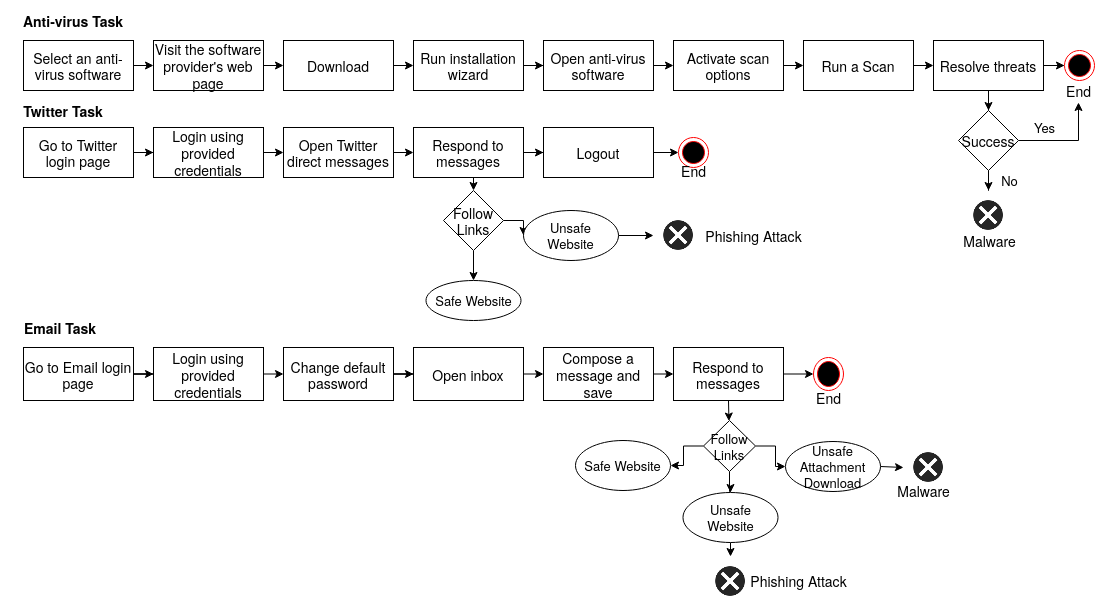
\includegraphics[width=1.1\columnwidth, keepaspectratio=true]{img/tasks.png}
  \caption{Sandbox task breakdown}
  \label{fig:tasks}
\end{figure}

\subsubsection{Self-efficacy}
The anti-virus task consisted of three sub-tasks: (1) given a legitimate and an illegitimate antivirus software, the user was asked to choose one (choice), (2) install the selected software and configure it to be used in the computer (install) and (3) run the software on the computer and remove threats (scan). In the post-survey, question 4 measures self-efficacy of the choice, question 9 measures the self-efficacy of the install and question 6 measures the self-efficacy of the scan. From the 62 participants only 11 completed all three sub-tasks, while 32 participants skipped the anti-virus task altogether. Those who did not complete the task skipped the install or scan or both. All 11 participants who completed all three sub-tasks installed the legitimate anti-virus software. This shows that users who practice computer security typically execute similar actions when they are placed in similar situations.

Listed below are the three questions we provided for the participants to  subjectively rate their efficacy to use Antivirus software.
Within parenthesis next to each subjective rating value is the numerical score we assigned for that particular rating.
When computing the mean efficacy for an activity in the Completed group, we sum the numerical scores of the subjective ratings given by the participants and divide by the number of participants in the Completed group who have answered that question.
For example assume three participants in the Completed group rated the efficacy of the Choice task as $[$ \textit{Neutral}, \textit{Disagree}, \textit{Agree} $]$.
Then, the mean efficacy for the Choice task in the Completed group is $\frac{3 + 2 + 4}{3} = 3$.
The mean efficacy for an activity in the Incomplete group is calculated similarly.
\begin{itemize}
\item (\textbf{efficacy of choice}) I feel confident in my ability to select an antivirus software that matches my security requirements.
\par Strongly Disagree (1) \hspace{0.5cm} Disagree (2)\hspace{0.5cm}Neutral (3)\hspace{0.5cm} Agree (4)\hspace{0.5cm} Strongly agree (5)
\item (\textbf{efficacy of install}) I choose an antivirus software, which allows me to customize its features to match my security requirements.
\par Strongly Disagree (1) \hspace{0.5cm} Disagree (2)\hspace{0.5cm}Neutral (3)\hspace{0.5cm} Agree (4)\hspace{0.5cm} Strongly agree (5)
\item (\textbf{efficacy of scan}) I feel confident in my ability to identify and remove suspicious files on my computer using an antivirus software without help.
\par Strongly Disagree (1) \hspace{0.5cm} Disagree (2)\hspace{0.5cm}Neutral (3)\hspace{0.5cm} Agree (4)\hspace{0.5cm} Strongly agree (5)
\end{itemize}
Table \ref{tab:avefficacy} shows the result of the two-tailed T-test that compares the self-reported efficacy between those who completed the choice task and those who did not is significant (P < 0.05). 
The same can be observed for the scan activity. 
However, the self-reported efficacy is not significant for the install task. This shows that for certain tasks that involve anti-virus software usage, users can incorrectly assess their self-efficacy when practicing computer security in self-reports.

\begin{table}[tpb]
\caption{Self reported self-efficacy differences between those who completed all anti-virus sub-tasks and those who did not complete the task.}
\label{tab:avefficacy}
\begin{tabular}{|l|l|l|l|}
\hline
Activity & \begin{tabular}[c]{@{}l@{}}Completed \\ Efficacy Mean (SD)\end{tabular} & \begin{tabular}[c]{@{}l@{}}Incomplete \\ Efficacy Mean (SD)\end{tabular} & P \\ \hline
Choice  & 4.181 (0.603) & 2.944 (0.998) & 0.00096 \\
Install & 3.6 (1.055)   & 3.428 (0.851) & 0.636   \\
Scan    & 4.0 (0.707)   & 2.875 (1.147) & 0.005   \\ \hline
\end{tabular}
\end{table}

Our post survey contained 3 questions (questions 14 - 16), which evaluated self efficacy of communicating safely on Twitter. 
As seen in Figure \ref{fig:tasks} the Twitter task contained the least number of steps. Furthermore, the action ``Respond to messages'' is a repetitive action. The action makes the user to read and respond to the three messages in their Twitter inbox. All 61 participants who completed the task opened/responded to at least one of the three messages.
Listed below are the three questions we provided for the participants to  subjectively rate their efficacy to use Twitter safely.
Within parenthesis next to each subjective rating value is the numerical score we assigned for that particular rating.
\begin{itemize}
\item (\textbf{Question 14}) I feel confident in my ability to identify suspicious messages on Twitter.
\par Strongly Disagree (1) \hspace{0.5cm} Disagree (2)\hspace{0.5cm}Neutral (3)\hspace{0.5cm} Agree (4)\hspace{0.5cm} Strongly agree (5)
\item (\textbf{Question 15}) I feel confident in my ability to identify suspicious messages on Twitter without help.
\par Strongly Disagree (1) \hspace{0.5cm} Disagree (2)\hspace{0.5cm}Neutral (3)\hspace{0.5cm} Agree (4)\hspace{0.5cm} Strongly agree (5)
\item (\textbf{Question 16}) I feel confident in my ability to identify suspicious messages on Twitter even if it is the first time I had seen one.
\par Strongly Disagree (1) \hspace{0.5cm} Disagree (2)\hspace{0.5cm}Neutral (3)\hspace{0.5cm} Agree (4)\hspace{0.5cm} Strongly agree (5)
\end{itemize}
\begin{table}[tpb]
\caption{Self reported self-efficacy means (standard deviation in parenthesis) between those who visited the phishing link and did not visit the phishing link during the Twitter task}
\label{tab:twitvisitedphishing}
\begin{tabular}{|l|l|l|l|}
\hline
Question &
  \begin{tabular}[c]{@{}l@{}}Mean (SD)\\ Visited phishing \\ link\end{tabular} &
  \begin{tabular}[c]{@{}l@{}}Mean (SD)\\ Did not visit\\ phishing link\end{tabular} &
  P \\ \hline
14 & 4.31 (0.87) & 4.04 (0.85) & 0.298 \\
15 & 4.13 (1.20) & 3.93 (0.96) & 0.571 \\
16 & 4.31 (0.87) & 3.84 (0.85) & 0.075 \\ \hline
\end{tabular}
\end{table}
Table \ref{tab:twitvisitedphishing} shows the result of the two-tailed T-test that compares the self-reported efficacy between those who visited the phishing web page following the link that appeared on their Twitter direct message and those who did not. 
We compute separate p-values for each question that asks the user to rate their self-efficacy. 
It can be seen that the participants evaluated their self efficacy to recognize phishing attempts while communicating on Twitter higher than it actually was. 
There is no significant difference between the self-efficacy ratings participants who clicked the phishing link and the participants who did not, P > 0.05 for all questions in Table \ref{tab:twitvisitedphishing}.

\begin{table}[tpb]
\caption{Self reported self-efficacy means (standard deviation in parenthesis) between those who visited the phishing site and did not submit their passwords and those who visited the site and submitted their passwords while using Twitter. P value is the two-tailed T-test}
\label{tab:twitvisitedphishingpass}
\begin{tabular}{|l|l|l|l|}
\hline
Question & \begin{tabular}[c]{@{}l@{}}Mean (SD)\\ Visited-No Password\end{tabular} & \begin{tabular}[c]{@{}l@{}}Mean (SD)\\ Visited-Yes Password\end{tabular} & P \\ \hline
14 & 4.25 (0.9) & 4.02 (0.85) & 0.335 \\
15 & 4.25 (0.9) & 3.90 (0.97) & 0.316 \\
16 & 4.25 (0.9) & 3.80 (0.84) & 0.305 \\ \hline
\end{tabular}
\end{table}

A similar observation can be made for the situation where the participant visited the phishing site and submitted their password information when using Twitter. 
Questions 14, 15 and 16 are also used to collect the self-efficacy subjective ratings for this task.
Table \ref{tab:twitvisitedphishingpass} shows that although there is no statistically significant difference between self reported self-efficacy ratings for the participants who visited the phishing site and also submitted their password and those visited the site but did not submit the password.
The phishing task has different risk levels.
Visiting the phishing website has a lower risk level compared to visiting the website and submitting the password.
Users who submitted the password to the phishing site further compromised their security by enabling the attacker to steal private information.

Users found it difficult to correctly assess their self-efficacy in practicing caution while communicating with email. 
Questions 21 and 22 in the post-survey asked users to rate their self efficacy. 
Within parenthesis next to each subjective rating value is the numerical score we assigned for that particular rating.
\begin{itemize}
\item (\textbf{Question 21}) I practice caution when responding to email from senders I am not familiar with.
\par Strongly Disagree (1) \hspace{0.5cm} Disagree (2)\hspace{0.5cm}Neutral (3)\hspace{0.5cm} Agree (4)\hspace{0.5cm} Strongly agree (5)
\item (\textbf{Question 22}) I practice caution downloading attachments in emails from senders I am not familiar with.
\par Strongly Disagree (1) \hspace{0.5cm} Disagree (2)\hspace{0.5cm}Neutral (3)\hspace{0.5cm} Agree (4)\hspace{0.5cm} Strongly agree (5)
\end{itemize}
When encountered with an email containing a phishing link, two tailed T-test showed that there is no statistical significance between self-efficacy ratings given by users who did not follow the phishing link compared to the users who did (P > 0.05). 
All who visited the phishing link, with the exception of one participant,  submitted their login username and the password to the phishing web site. 
The users who submitted their login username and the password had a mean self-efficacy rating 3.89 (SD=0.90). 
Similar observation can be made from users who downloaded malicious attachments that come with email. Two tailed T-test revealed that there is no statistical significance (P > 0.05) between the self-efficacy ratings given by users who downloaded malicious attachments  from email against the users who did not.

\subsubsection{Cues-to-Action}
We focus on cues that are available on the computer system to evaluate how cues-to-action affect the user's computer security behavior. For the anti-virus usage task, we focused on two cues: (1) whether or not the download page was secure (has HTTPS with SSL lock icon), and (2) software provider/web page appears to be legitimate (look and feel, content etc.). Secure download was tested with post-survey question 29 and legitimate provider cue was tested with post-survey question 8. The Twitter task cues were tested with questions 17, 18, 19, 26. We considered cues such as: (1) unknown sender, (2) suspicious message content, (3)shortened URL links that appear in twitter messages and (4) secure HTTPS Twitter login page. For the email task we used two cues: (1) secure HTTPS web pages and (2) Firefox expired certificate warning. The post-survey questions 20 and 28 evaluated whether or not users picked up on these cues for email.

Listed below are the questions we provided for the participants to  subjectively rate their ability to detect cues-to-action when using the Twitter application.
Within parenthesis next to each subjective rating value is the numerical score we assigned for that particular rating.
\begin{itemize}
\item (\textbf{Question 17}) Before following a link on Twitter, I first check if it was sent by an unknown sender or contains suspicious information.
\par Strongly Disagree (1) \hspace{0.5cm} Disagree (2)\hspace{0.5cm}Neutral (3)\hspace{0.5cm} Agree (4)\hspace{0.5cm} Strongly agree (5)
\item (\textbf{Question 18}) I practice caution when I follow links sent to me on messages on Twitter as they may expose me to a security threat.
\par Strongly Disagree (1) \hspace{0.5cm} Disagree (2)\hspace{0.5cm}Neutral (3)\hspace{0.5cm} Agree (4)\hspace{0.5cm} Strongly agree (5)
\item (\textbf{Question 19}) I do not follow links sent to me on Twitter messages, if the content looks suspicious.
\par Strongly Disagree (1) \hspace{0.5cm} Disagree (2)\hspace{0.5cm}Neutral (3)\hspace{0.5cm} Agree (4)\hspace{0.5cm} Strongly agree (5)
\item (\textbf{Question 26}) Was Twitter.com page you saw during the experiment a secure web page?
\par Yes \hspace{1cm} No \hspace{1cm} I do not know
\end{itemize}

Listed below are the questions we provided for the participants to  subjectively rate their ability to detect cues-to-action when using email.
\begin{itemize}
\item (\textbf{Question 20}) When I see a message warning me about the security of a web site (e.g., expired certificate, http:// instead of https://) I am about to visit, I do not visit that web site.
\par Strongly Disagree \hspace{1cm} Disagree\hspace{1cm}Neutral\hspace{1cm} Agree\hspace{1cm} Strongly agree
\item (\textbf{Question 28}) When you submit private information (passwords, email addresses) to websites, do you verify that the site is secure and your information is safe?
\par Yes \hspace{1cm} No \hspace{1cm} I do not know
\end{itemize}

In the anti-virus task, we used user responses to question 8 to compare self-reports of ability to recognize safety of anti-virus software by looking at the provider's web page.
\begin{itemize}
\item (\textbf{Question 8}) Before choosing a source to download software, I first check if it is hosted by a trustworthy provider as it may expose me to a security threat.
\par Strongly Disagree (1) \hspace{0.5cm} Disagree (2)\hspace{0.5cm}Neutral (3)\hspace{0.5cm} Agree (4)\hspace{0.5cm} Strongly agree (5)
\end{itemize}
Participants' mean self-report value was 3.86 (SD=0.94) for the safe software and 3.00 (SD=1.00) for the unsafe software. 
Two tailed, T-test between the users who selected the safe software vs. the unsafe software showed that the mean difference is significant (P < 0.05). This allows us to conclude that the web page content cue helps users to select a safe anti-virus software. 
Listed below are is the question we provided for the participants to  subjectively rate their ability to detect cues-to-action to recognize secure web sites when downloading software from the Internet.
The specific cue we are checking is the HTTPS URL with the padlock icon on the browser address bar.
\begin{itemize}
\item (\textbf{Question 29}) During the experiment did you download the antivirus software from a secure web page?
\par Yes \hspace{1cm} No \hspace{1cm} I do not know
\end{itemize}
Question 29 had categorical responses. 
We used the Chi-square test of independence to determine whether the HTTPS cue is associated with users selecting a safe software. 
Results showed we can reject the null hypothesis that the HTTPS cue is not associated with users selecting safe software (P=0.002, df=2).

In the Twitter task question 17 evaluated the unknown sender cue. Question 18 evaluated the shortened URL links in the message cue. Question 19 evaluated the suspicious message content cue. Question 26 evaluated the HTTPS with SSL padlock icon cue. Two tailed T-test for ability to recognize cues for questions 17, 18 and 19 between participants who visited the phishing link and participants who did not were not significant (P > 0.05). Question 26 contained categorical responses. We used the Chi-square test of independence to determine whether the HTTPS cues is associated with user with users following unsafe links on Twitter. Results showed we can not reject the null hypothesis that the HTTPS cue is not associated with users following unsafe links on Twitter (P=0.84, df=2).

In the email task question 20 evaluated the cue of the expired certificate warning generated by the browser when following a link. Question 28 evaluated the HTTPS cue, when submitting personal information to web sites. Two tailed T-test for ability to recognize cues for questions 20 between participants who followed a link to visit an unsafe website and those who did not was not significant. Participants' mean self-report value was 3.47 (SD=0.77) for those who visited the unsafe site and 3.82 (SD=0.88) for those who did not visit the unsafe site. Question 28 contained categorical responses. We used the Chi-square test of independence to determine whether the HTTPS cues is associated with user with users submitting personal information to web sites. Results showed we can not reject the null hypothesis that the HTTPS cue is not associated with users submitting personal information to websites (P=0.85, df=2).


\section{Discussion}
The results of our study validate the conclusions in previous studies, which states that human users' security related behavior often does not match their stated intentions \cite{davinson2010, govani2005, national2010}. 
For the software installation tasks, the Twitter task and the email task, the participants overestimated their efficacy to recognize undesirable consequences. This shows that the home computer users do not think about the post conditions of the actions they execute in the computer and therefore can benefit from an intervention system that help them identify actions leading to undesirable consequences.
Furthermore, the cues-to-action we have discussed in this study are preconditions that exist in the computer system. 
For example, identifying whether the web page the user is visiting contains the HTTPS SSL padlock icon, or whether the user is opening an email sent by an unknown (not in address book) sender are preconditions that can be checked by  the human user before completing the task (downloading software, clicking a link on the email).
Although we expect human users to recognize the preconditions (cues) leading to undesirable consequences all the time, this study concludes that it is not the case. 
We found that the users can recognize certain preconditions that exist in the system (e.g., the web page that they are visiting to download a software is secure) to help them avoid undesirable consequences. 
However, in other situations they miss these cues (e.g., recognizing unsafe web pages on Twitter) and as a result may end up compromising security.
Therefore, the design of software to assist home computer users in avoiding security and privacy vulnerabilities should be motivated by careful studies of their behavior and perceptions.

PsychoRithm sandbox environment allowed us to place human users in simulated scenarios that compromised their security/privacy and record their actual responses and at the same time capture the self-reported data on how users perceive their confidence in identifying risky situations (self-efficacy) and recognize cues that indicate danger (cues-to-action). Although, we are measuring factors that affect the computer security behavior of users (extracted from the Health Belief Model), our objective in this study is not to validate the model, but rather highlight that regardless the perceived self-efficacy and availability of cues, human users can still end up compromising their security. 
When the threat is immediate, if the user is not interrupted they may end up putting their safety at even more risk. 
To this end, the intervention models presented in this dissertation target helping human users avoid undesirable consequences.

In this study we mainly looked at three common home computer user tasks:
\begin{itemize}
\item Using anti-virus software to secure the computer
\item Communicating with Twitter direct messages
\item Using email
\end{itemize}

By analyzing the results, we identified important conditions that should be addressed when designing an intervention system to help human users. First, even though users were given step-by-step instructions for completing these tasks, they rarely follow the script. 
The users repeated the same action multiple times, while some actions were omitted altogether. 
The implication of this observation is that intervention systems that monitor users to help them avoid unsafe consequences need to handle noisy and/or missing actions in the observations.
Furthermore, any partially complete task (i.e., a sequence of actions) that has been safe upto now may quickly turn unsafe. 
This means that the intervention decisions need to be made online. 
Users perform a large number of actions; while few of them incur much risk, some are pivotal in triggering vulnerabilities. For example, from our using email task, opening email action itself is not a risky action. 
However, when the email is from an unknown sender and contains suspicious attachments, preconditions to a malware vulnerability have manifested within the system. In this state,  opening email is actually high risk action.
This means that intervention models need to search for multiple ways for accomplishing the same task. Modeling the problem as a state/action transition system using automated planning allows us to accomplish this requirement. When the problem is modeled as a planning domain, automated planners can be used to generate diverse plans, to sample the space of possible plans that can lead to one or more vulnerabilities and help
estimate the probability that particular actions lead to triggering the vulnerabilities.


Second, the objective of the intervention system will be to identify when a user's action(s) may be complicit in triggering the threats and help the user avoid the undesirable state (security or privacy breach).
Given a fine-grained model of user and attacker actions and states of the system as an automated planning domain, the intervention system should be able to identify actions that can lead to triggering a vulnerability.
A previous study \cite{byrne2016} showed that users pay more attention to the benefits of the activities than the risk; they have goals that they want/need to achieve and are willing to take the risk to achieve them. 
Many triggering actions may be normal activities (e.g., reading email, clicking on links)
with the user more focused on the goal than on the risk.
Thus, the undesirable consequence recognition problem needs to take into account the user's intention as well as the undesirable consequence.
Undesirable consequences prediction is assessing whether an action is likely to lead to undesirable consequences, immediately or as part of an action sequence, or may provide conditions
that an attacker can exploit. 
User intentions recognition determines what the user is intending to do through his/her actions, the short or long term goals.
The intervention decision involves a trade-off in early recognition of potential danger of an action versus the certainty that the effects will occur. In the chapters that follow we examine how different metrics captured from the planning problem representation can be used to assess that trade-off.
To help the user trade-off benefits versus risks, we also need to know what the user thinks he/she
is trying to accomplish. In some cases the goal may be explicitly stated in terms of actions and post-conditions. In other cases, the user's goal may be unknown. We consider both these conditions in the intervention models we present.


Third, personalization becomes most important when the intervention system must decide how to prevent an imminent security/privacy threat or decide what to do when one has been detected. Simply preventing a user from doing something they want to do will undoubtedly result in the security software being disabled. 
Our underlying hypothesis is that security will be more effective when the user is a partner with the system in the security interventions. In Chapter 6 of this dissertation, we present an intervention model designed for human users that uses automated planning to guide the user away from the undesirable consequence by giving hints.



\section{Concluding Remarks}
The design of software to assist home computer users in avoiding security and privacy vulnerabilities should be motivated by careful studies of their behavior and perceptions.
In this work, we created sandbox software to simulate, in a protected environment,
the user interface to an operating system and browser so that we could capture subject actions related to security and privacy in a realistic setting. 
Each subject took an initial survey to assess demographics, computer self-efficacy and perceptions of security/privacy, then used the simulator to ``setup and test basic functionality in a recently purchased computer'' (the cover story) and then took a survey to assess their perceptions of what they had done. 
In our analysis, we found that the users (adults taking a psychology course in Colorado State University) are unaware when they have made poor decisions and have triggered vulnerabilities. 
In the following chapters we present intervention models designed to automatically detect when such situations occur, i.e., that a user’s action(s) may be contributing to triggering a security or privacy threat.
To identify pivotal events, the appropriate system states and user actions must be monitored and compared to a model of actions that can lead to triggering a vulnerability.
We use automated planning to model the actions in environments where the user's decision making context differs in terms of what the user knows about the domain and the type of observational data available to identify pivotal events.

If an action that contributes to a trigger is suspected, it should be put in the context of what the user is trying to do and an estimate of how likely the action is to actually trigger the vulnerability.
Therefore, future studies for developing tools to help human users practice cyber-security must employ surveys, sandbox simulations and lightweight in situ monitoring to accurately understand the human users' decision making context. 
While the sandbox offers a controlled environment, in situ affords realism and the ability to conduct longitudinal studies. Therefore, lightweight tools need to be developed for unobtrusively monitoring the user and logging actions related to security. Longitudinal evaluation of intervention techniques is important to determine whether the new techniques will eventually be susceptible to
habituation (a major issue with current intervention techniques) and to examine if user’s actions change over time as security awareness increases.

In this study, we only analyzed two specific user traits: self-efficacy, and cues to action when we presented the user with choices of anti-virus software to install and asked them to do ordinary tasks like reading/sending email and reading/responding to tweets.
Future studies need to extend the state/action model of the home computer environment by including more scenarios and attacker actions.
Although self-efficacy and cues to action capture important aspects of the user's decision making context in the home computing environment: post-conditions and pre-conditions of actions the user executes respectively, there are many other factors that can define the decision making context of a human user (e.g., computer experience, decision-making psychometrics, risk aversion, perceived social status, the need
to belong). Developing realistic scenarios that capture these additional traits to study human user behavior in security situations is a challenging yet critical step in developing more personalizable intervention models.



